%%%%%%%%%%%%%%%%%%%%%%%%%%%%%%%%%%%%%%%%%%%%%%%%%%%%%%%%%%%%%%%%%%%%%%
%% Risk-Optimal Momentum Weights for Stochastic Gradient Estimation  %%
%% in High Dimensions                                                %%
%%                                                                   %%
%% Springer Nature LaTeX template, sn-jnl.cls                        %%
%%%%%%%%%%%%%%%%%%%%%%%%%%%%%%%%%%%%%%%%%%%%%%%%%%%%%%%%%%%%%%%%%%%%%%

\documentclass[pdflatex,sn-mathphys-num]{sn-jnl}% Math and Physical Sciences Numbered Reference Style

\usepackage{graphicx}%
\usepackage{multirow}%
\usepackage{amsmath,amssymb,amsfonts}%
\usepackage{amsthm}%
\usepackage{mathrsfs}%
\usepackage[title]{appendix}%
\usepackage{xcolor}%
\usepackage{textcomp}%
\usepackage{manyfoot}%
\usepackage{booktabs}%
\usepackage{algorithm}%
\usepackage{algorithmicx}%
\usepackage{algpseudocode}%
\usepackage{subcaption}
\usepackage{bm}

\theoremstyle{thmstyleone}%
\newtheorem{theorem}{Theorem}%
\newtheorem{proposition}[theorem]{Proposition}%
\newtheorem{corollary}[theorem]{Corollary}%

\theoremstyle{thmstyletwo}%
\newtheorem{example}{Example}%
\newtheorem{remark}{Remark}%
\newtheorem{lemma}{Lemma}%

\theoremstyle{thmstylethree}%
\newtheorem{definition}{Definition}%

%%%%%%%%%%%%%%%%%%%%%%%%%%%%%%%%%%%%%%%%%%%%%%%%%%%%%%%%%%%%%%%%%%%%%%
%% ATTENTION.  The macro below marks every number in the image        %%
%% classification section that must be replaced by the output of the  %%
%% re-run of that grid with the algorithm of this paper.  Search the  %%
%% source for \torerun before submitting; the manuscript is not ready %%
%% while any occurrence remains.  The run commands are listed in the  %%
%% comment block at the head of that section.                         %%
%%%%%%%%%%%%%%%%%%%%%%%%%%%%%%%%%%%%%%%%%%%%%%%%%%%%%%%%%%%%%%%%%%%%%%
\newcommand{\torerun}[1]{\textcolor{red}{\textbf{[#1]}}}

\newcommand{\peff}{p_{\mathrm{eff}}}
\newcommand{\tr}{\mathrm{tr}}
\newcommand{\Var}{\mathrm{Var}}
\newcommand{\Cov}{\mathrm{Cov}}
\newcommand{\diag}{\mathrm{diag}}
\newcommand{\E}{\mathbb{E}}
\newcommand{\Real}{\mathbb{R}}

\raggedbottom

\begin{document}

\title[Risk-Optimal Momentum Weights for Stochastic Gradient Estimation]{Risk-Optimal Momentum Weights for Stochastic Gradient Estimation in High Dimensions}

\author*[1]{\fnm{Mohammad} \sur{Arashi}}\email{arashi@um.ac.ir}
\equalcont{These authors contributed equally to this work.}

\author[2]{\fnm{Mahmood} \sur{Amintoosi}}\email{m.amintoosi@um.ac.ir}
\equalcont{These authors contributed equally to this work.}

\affil*[1]{\orgdiv{Department of Statistics, Faculty of Mathematical Sciences}, \orgname{Ferdowsi University of Mashhad}, \orgaddress{\street{P.O. Box 1159}, \city{Mashhad}, \postcode{91775}, \country{Iran}}}

\affil[2]{\orgdiv{Division of Computer Science, Department of Applied Mathematics, Faculty of Mathematical Sciences}, \orgname{Ferdowsi University of Mashhad}, \orgaddress{\street{P.O. Box 1159}, \city{Mashhad}, \postcode{91775}, \country{Iran}}}

\abstract{Adaptive stochastic gradient methods form their search direction by averaging the current mini-batch gradient with a running average of past gradients, using a weight fixed in advance by a decay hyperparameter. We show that this direction is exactly a shrinkage estimator of the population gradient, with a deterministic weight, and we ask what weight minimises its conditional quadratic risk. The answer is a positive-part Stein rule whose constant is set by the dimension of the parameter block and whose statistic is the current gradient standardised by the coordinatewise gradient-noise variance. We give a dominance theorem that covers heteroscedastic noise, an estimated scale matrix and an arbitrary diagonal loss weighting in one statement, and we show that the loss weighting decides whether the nominal dimension or an effective dimension governs the admissible constant. Because the rule needs a variance estimate, we analyse the natural candidate built from the moments an adaptive optimiser already maintains, and we prove that it is biased by a factor we compute in closed form for every iteration, which yields an exactly unbiased correction. Under elliptically contoured gradient noise the dominance window contracts by an explicitly computable factor, equal to one minus twice the reciprocal degrees of freedom for the multivariate Student law. The resulting algorithm, SR-Adam, is analysed as a biased stochastic approximation and converges at the usual non-convex rate up to a floor set by the largest coordinatewise gradient-noise variance of the block, hence inversely proportional to the batch size. Monte Carlo studies confirm every constant, and controlled optimisation experiments show gains that grow with the gradient-noise level.}

\keywords{Stein-rule estimation, Stochastic gradient methods, Shrinkage, Decision theory, High-dimensional inference, Adaptive optimisation}

\maketitle

%%%%%%%%%%%%%%%%%%%%%%%%%%%%%%%%%%%%%%%%%%%%%%%%%%%%%%%%%%%%%%%%%%%%%%
\section{Introduction}
\label{sec:introduction}

The inadmissibility of the sample mean in three or more dimensions is one of the organising results of statistical decision theory. Stein \cite{stein1956} and James and Stein \cite{james1961} showed that the usual estimator of a multivariate normal mean is dominated under quadratic loss once the dimension reaches three, and the estimators that dominate it trade a small bias for a larger reduction in variance. Sixty years of subsequent work has mapped the boundaries of that phenomenon, from the minimax families of Baranchik \cite{baranchik1970} and Bock \cite{bock1975} through the unbiased risk estimate of Stein \cite{stein1981} to the spherically symmetric theory of Strawderman \cite{strawderman1974}, Brandwein and Strawderman \cite{brandwein1990, brandwein2012} and Cellier and Fourdrinier \cite{cellier1995, cellier1995b}, and the modern accounts of Berger \cite{berger1985}, Lehmann and Casella \cite{lehmann1998}, Fourdrinier, Strawderman and Wells \cite{fourdrinier2018} and Saleh \cite{saleh2006}. The empirical Bayes reading of the phenomenon due to Efron and Morris \cite{efronmorris1973, efronmorris1976, efron2012} is the one closest in spirit to what follows, since the weight the rule selects is an estimate of a posterior shrinkage factor. Related ideas drive thresholding in sparse settings \cite{donoho1994}, covariance regularisation \cite{ledoit2004} and penalised regression \cite{saleh2019}.

Training a modern neural network is a high-dimensional estimation problem of exactly this shape, repeated many times. At each iteration the optimiser observes a mini-batch gradient, treats it as a noisy reading of the population gradient, and forms a search direction. The dominant methods build that direction by exponential averaging. Momentum \cite{polyak1964, sutskever2013} averages past gradients; AdaGrad \cite{duchi2011}, RMSProp \cite{tieleman2012} and Adam \cite{kingma2015} add a coordinatewise rescaling driven by a second moment. These constructions are justified by optimisation arguments rather than by statistical risk, and the averaging weight is a hyperparameter chosen once and held fixed for the whole run.

That last point is the opening this paper works through. Writing $\hat{\bm m}_t$ for the bias-corrected first moment that Adam maintains, an elementary identity, recorded as Lemma \ref{lem:adam_identity} below, gives
\begin{equation}
\label{eq:adam_convex}
\hat{\bm m}_t
=
\hat{\bm m}_{t-1}
+
w_t\bigl(\bm g_t-\hat{\bm m}_{t-1}\bigr),
\qquad
w_t=\frac{1-\beta_1}{1-\beta_1^{t}} .
\end{equation}
The Adam direction is therefore a convex combination of the current gradient and the historical average, that is, a shrinkage estimator of the population gradient that shrinks the noisy current reading toward a stable reference. Its weight is deterministic and is fixed by $\beta_1$. The question this paper answers is what weight a decision-theoretic analysis would put in its place, what can be proved about the resulting estimator when the ingredients it needs are themselves estimated from data, and what the substitution does to the behaviour of the optimiser.

The highlights of our contribution are as follows. 
\begin{itemize}

\item The search direction of an adaptive gradient method is a shrinkage estimator whose weight is fixed by a hyperparameter, and we replace that weight by the one minimising conditional quadratic risk.

\item One dominance theorem covers heteroscedastic noise, a scale matrix estimated from the past and an arbitrary diagonal loss weighting together, where existing statements treat them separately.

\item The loss weighting, not the covariance, decides which dimension bounds the admissible shrinkage constant, the nominal parameter count under the standardised loss and a smaller effective dimension otherwise.

\item The variance estimate an adaptive optimiser forms from its own moments is biased by a factor we compute in closed form at every iteration, which yields an exactly unbiased correction.

\item Under elliptically contoured noise the dominance window contracts by a factor we identify exactly, equal to $(\nu-2)/\nu$ for multivariate Student noise with $\nu$ degrees of freedom.

\item The shrinkage displacement obeys a sharp deterministic bound, which yields a non-asymptotic convergence statement for a deliberately biased direction with an explicit floor that is inversely proportional to the batch size.

\end{itemize}

Every constant claimed above is confirmed numerically in Section \ref{sec:simulation}, and the code that produces the confirmation accompanies the paper.

\subsection{Relation to earlier work}

Stochastic approximation begins with Robbins and Monro \cite{robbins1951}, and the modern non-convex theory is set out by Nemirovski and coauthors \cite{nemirovski2009}, Ghadimi and Lan \cite{ghadimi2013} and Bottou, Curtis and Nocedal \cite{bottou2018}, with the dynamical-systems treatment of Borkar \cite{borkar2008} and Kushner and Yin \cite{kushner2003} supplying the almost sure route. Variance reduction in stochastic optimisation is usually pursued through control variates that exploit finite-sum structure, as in the methods of Johnson and Zhang \cite{johnson2013} and Defazio, Bach and Lacoste-Julien \cite{defazio2014}. Those methods reduce variance without introducing bias and require periodic full-gradient evaluations. The route taken here is different in kind, since it accepts bias in exchange for a larger variance reduction and needs nothing beyond the moments an adaptive optimiser already stores.

On the analysis side, convergence guarantees for Adam-type methods have been established under bounded-gradient conditions by Reddi, Kale and Kumar \cite{reddi2018}, Chen, Liu, Sun and Hong \cite{chen2019}, Zaheer and coauthors \cite{zaheer2018}, Barakat and Bianchi \cite{barakat2021}, and D\'efossez and coauthors \cite{defossez2022}. All of these treat the search direction as an unbiased gradient estimate up to the preconditioner. The estimator studied here is deliberately biased, so those arguments do not transfer, and Section \ref{sec:convergence} supplies a biased-stochastic-approximation analysis instead.

On the noise side, the Gaussian working model for mini-batch gradients goes back to the diffusion approximations of Mandt, Hoffman and Blei \cite{mandt2017}. Evidence that the noise is heavier tailed than Gaussian has been assembled by Simsekli, Sagun and Gurbuzbalaban \cite{simsekli2019}, Panigrahi and coauthors \cite{panigrahi2019}, Zhang and coauthors \cite{zhang2020attention}, and Gurbuzbalaban, Simsekli and Zhu \cite{gurbuzbalaban2021}, and it is the same evidence that motivates gradient clipping \cite{zhang2020clipping}. Section \ref{sec:elliptical} responds to that evidence by replacing the Gaussian assumption with an elliptical one and tracking what the replacement costs.

\subsection{Organisation}

Section \ref{sec:setup} fixes notation and assumptions and records the identity \eqref{eq:adam_convex}. Section \ref{sec:risk} develops the risk theory, Section \ref{sec:elliptical} relaxes normality, and Section \ref{sec:variance} treats variance estimation. Section \ref{sec:algorithm} assembles the algorithm and Section \ref{sec:convergence} analyses its convergence. Section \ref{sec:simulation} reports the Monte Carlo studies, Section \ref{sec:experiments} the image classification experiments, and Section \ref{sec:conclusion} discusses limitations and directions. Proofs are collected in Appendix \ref{sec:proofs}.

%%%%%%%%%%%%%%%%%%%%%%%%%%%%%%%%%%%%%%%%%%%%%%%%%%%%%%%%%%%%%%%%%%%%%%
\section{Setup and assumptions}
\label{sec:setup}

Let $(\Omega,\mathcal F,\mathbb P)$ be a complete probability space carrying all random elements below. The objective is
\begin{equation}
J(\bm\theta)=\E_{x\sim\mathcal D}\bigl[L(x,\bm\theta)\bigr],
\qquad
\bm\theta\in\Real^{p},
\end{equation}
and the optimiser produces iterates $\bm\theta_1,\bm\theta_2,\dots$ driven by mini-batch gradients $\bm g_1,\bm g_2,\dots$. Set $\mathcal F_0=\sigma(\bm\theta_1)$ and $\mathcal F_t=\sigma(\bm\theta_1,\bm g_1,\dots,\bm g_t)$ for $t\ge1$, so that $\bm\theta_t$ is $\mathcal F_{t-1}$-measurable by construction. Vectors are column vectors, $\|\cdot\|$ is the Euclidean norm, $\|\cdot\|_\infty$ the supremum norm, and for a positive definite diagonal $\bm D$ we write $\|\bm x\|^2_{\bm D}=\bm x'\bm D\bm x$. For a diagonal positive definite $\bm\Sigma$ we write $\lambda_{\max}(\bm\Sigma)$ for its largest entry.

In a network the parameter vector is partitioned into blocks, one per weight tensor, and every construction below is applied blockwise. To keep the notation light we suppress the block index and write $p$ for the dimension of the block under discussion.

The standing assumptions are the following.

\begin{itemize}
\item[(A1)] $J$ is continuously differentiable, bounded below by $J^\star$, and $\nabla J$ is Lipschitz with constant $L$.
\item[(A2)] Conditionally on $\mathcal F_{t-1}$ the mini-batch gradient satisfies $\bm g_t=\nabla J(\bm\theta_t)+\bm\varepsilon_t$ with $\E[\bm\varepsilon_t\mid\mathcal F_{t-1}]=\bm 0$ and $\Cov(\bm\varepsilon_t\mid\mathcal F_{t-1})=\bm\Sigma_t=\diag(\sigma^2_{t,1},\dots,\sigma^2_{t,p})$ positive definite.
\item[(A3)] Conditionally on $\mathcal F_{t-1}$ the noise is normal, $\bm\varepsilon_t\mid\mathcal F_{t-1}\sim\mathcal N_p(\bm 0,\bm\Sigma_t)$. Section \ref{sec:elliptical} replaces this by an elliptical assumption.
\item[(A4)] There are finite $G$ and $G_\infty$ with $\|\bm g_t\|\le G$ and $\|\bm g_t\|_\infty\le G_\infty$ almost surely for every $t$.
\item[(A5)] Over the window on which the variance estimator of Section \ref{sec:variance} is formed, each coordinate process $\{g_{t,j}\}$ is strictly stationary with finite fourth moment and serially uncorrelated, and the coordinatewise variance estimates satisfy $\sum_{k=1}^{p}\bigl|\Cov(\hat s^2_{t,j},\hat s^2_{t,k})\bigr|\le C$ uniformly in $j$ and $t$.
\end{itemize}

Assumption (A3) is the working model of the diffusion approximation literature \cite{mandt2017} and is the one under which the classical shrinkage results are stated. It is not a description of deep learning gradient noise, which is heavier tailed \cite{simsekli2019, gurbuzbalaban2021}, and Section \ref{sec:elliptical} is devoted to measuring the gap. Assumption (A4) is the bounded-gradient condition used throughout the convergence analysis of adaptive methods \cite{reddi2018, chen2019, defossez2022}. Assumption (A5) concerns only the sampling behaviour of the variance estimator, and Remark \ref{rem:a5} records what happens when the serial-uncorrelatedness part fails.

\subsection{The adaptive direction is a shrinkage estimator}

Adam maintains $\bm m_t=\beta_1\bm m_{t-1}+(1-\beta_1)\bm g_t$ with $\bm m_0=\bm 0$ and uses the bias-corrected $\hat{\bm m}_t=\bm m_t/(1-\beta_1^{t})$.

\begin{lemma}
\label{lem:adam_identity}
For every $t\ge1$ and $\beta_1\in[0,1)$,
\begin{equation}
\hat{\bm m}_t=\hat{\bm m}_{t-1}+w_t\bigl(\bm g_t-\hat{\bm m}_{t-1}\bigr),
\qquad
w_t=\frac{1-\beta_1}{1-\beta_1^{t}},
\end{equation}
with the convention $\hat{\bm m}_0=\bm 0$, so that $w_1=1$ and $\hat{\bm m}_1=\bm g_1$. The weight $w_t$ decreases monotonically from one to $1-\beta_1$.
\end{lemma}

Lemma \ref{lem:adam_identity} puts the whole family of directions
\begin{equation}
\label{eq:direction_family}
\bm d_t(k)=\hat{\bm m}_{t-1}+k\bigl(\bm g_t-\hat{\bm m}_{t-1}\bigr),
\qquad
k\in[0,1],
\end{equation}
on the table, with Adam occupying the single point $k=w_t$. Since $\hat{\bm m}_{t-1}$ is $\mathcal F_{t-1}$-measurable, the choice of $k$ is a choice of estimator of $\nabla J(\bm\theta_t)$ from the single observation $\bm g_t$. Writing
\begin{equation}
\label{eq:Ydelta}
\bm Y_t=\bm g_t-\hat{\bm m}_{t-1},
\qquad
\bm\delta_t=\nabla J(\bm\theta_t)-\hat{\bm m}_{t-1},
\end{equation}
assumption (A3) gives $\bm Y_t\mid\mathcal F_{t-1}\sim\mathcal N_p(\bm\delta_t,\bm\Sigma_t)$, and the conditional risk of $\bm d_t(k)$ under a diagonal loss weight $\bm D$ is
\begin{equation}
\label{eq:risk_reduces}
\E\Bigl[\bigl\|\bm d_t(k)-\nabla J(\bm\theta_t)\bigr\|^2_{\bm D}\;\Big|\;\mathcal F_{t-1}\Bigr]
=
\E\Bigl[\bigl\|k\bm Y_t-\bm\delta_t\bigr\|^2_{\bm D}\;\Big|\;\mathcal F_{t-1}\Bigr].
\end{equation}
The estimation problem has been reduced to the choice of $k$ in a normal location model. Two benchmarks follow at once. Taking $k=1$ recovers the raw mini-batch gradient, with conditional risk $\tr(\bm D\bm\Sigma_t)$. Minimising \eqref{eq:risk_reduces} over deterministic $k$ gives the oracle weight
\begin{equation}
\label{eq:oracle_weight}
k^{\mathrm{or}}_t=\frac{\|\bm\delta_t\|^2_{\bm D}}{\|\bm\delta_t\|^2_{\bm D}+\tr(\bm D\bm\Sigma_t)},
\end{equation}
which is unavailable because $\bm\delta_t$ is unknown. The Stein rule of the next section is a plug-in for \eqref{eq:oracle_weight}, and Section \ref{sec:simulation} shows that the two agree closely across the whole range of signal-to-noise ratios.

%%%%%%%%%%%%%%%%%%%%%%%%%%%%%%%%%%%%%%%%%%%%%%%%%%%%%%%%%%%%%%%%%%%%%%
\section{Risk theory for the shrinkage weight}
\label{sec:risk}

Throughout this section we condition on $\mathcal F_{t-1}$ and suppress the index $t$. The observation is $\bm Y\sim\mathcal N_p(\bm\mu,\bm\Sigma)$ with $\bm\Sigma=\diag(\sigma^2_1,\dots,\sigma^2_p)$. The rule uses a diagonal positive definite scale matrix $\bm A=\diag(a_1,\dots,a_p)$, which in the algorithm is an estimate of $\bm\Sigma$ formed from the past and is therefore a fixed matrix once we condition, and forms
\begin{equation}
\label{eq:Q_and_delta}
Q=\bm Y'\bm A^{-1}\bm Y,
\qquad
\hat{\bm\mu}_c(\bm Y)=\Bigl(1-\frac{c}{Q}\Bigr)\bm Y ,
\qquad c>0 .
\end{equation}
Risk is measured by $\|\cdot\|^2_{\bm D}$ for a diagonal positive definite $\bm D=\diag(d_1,\dots,d_p)$, also fixed given the past.

\subsection{A dominance theorem in one statement}

\begin{theorem}
\label{thm:master}
Let $p\ge3$ and let $\bm\Sigma$, $\bm A$ and $\bm D$ be diagonal and positive definite. Then $\E[Q^{-1}]<\infty$, the risk of $\hat{\bm\mu}_c$ satisfies the identity
\begin{equation}
\label{eq:master_identity}
\E\bigl\|\hat{\bm\mu}_c(\bm Y)-\bm\mu\bigr\|^2_{\bm D}
-\tr(\bm D\bm\Sigma)
=
\E\left[
-\frac{2c\,\tr(\bm D\bm\Sigma)}{Q}
+\frac{4c\,\bm Y'\bm D\bm\Sigma\bm A^{-1}\bm Y}{Q^{2}}
+\frac{c^{2}\,\bm Y'\bm D\bm Y}{Q^{2}}
\right],
\end{equation}
and consequently $\hat{\bm\mu}_c$ dominates $\bm Y$ under $\|\cdot\|^2_{\bm D}$ whenever
\begin{equation}
\label{eq:master_window}
0<c<\frac{2\bigl(\tr(\bm D\bm\Sigma)-2\max_{j}d_j\sigma^2_j\bigr)}{\max_{j}d_ja_j} .
\end{equation}
The right-hand side of \eqref{eq:master_window} is positive if and only if $\tr(\bm D\bm\Sigma)>2\max_{j}d_j\sigma^2_j$.
\end{theorem}

The identity \eqref{eq:master_identity} is exact and the window \eqref{eq:master_window} is sufficient rather than necessary, a distinction Section \ref{sec:simulation} makes visible by locating the empirical sign change of the risk difference. Four specialisations carry the argument of the paper.

\begin{corollary}
\label{cor:cases}
Under the conditions of Theorem \ref{thm:master} the following hold.
\begin{enumerate}
\item[(i)] With $\bm D=\bm I_p$, $\bm A=\bm\Sigma=\sigma^2\bm I_p$ and $\hat{\bm\mu}_c$ written as $(1-a/\|\bm Y\|^2)\bm Y$, dominance holds for $0<a<2(p-2)\sigma^2$, the classical James--Stein window.
\item[(ii)] With $\bm D=\bm I_p$ and $\bm A=\bm\Sigma$ heteroscedastic, dominance holds for $0<c<2(\peff-2)$, where
\begin{equation}
\peff=\frac{\tr\bm\Sigma}{\lambda_{\max}(\bm\Sigma)} .
\end{equation}
\item[(iii)] With $\bm D=\bm A^{-1}=\bm\Sigma^{-1}$, dominance holds for $0<c<2(p-2)$, whatever the heteroscedasticity of $\bm\Sigma$.
\item[(iv)] With $\bm D=\bm A^{-1}=\widehat{\bm\Sigma}^{-1}$ for an estimate $\widehat{\bm\Sigma}=\diag(\hat\sigma^2_1,\dots,\hat\sigma^2_p)$ formed from the past, and writing $r_j=\sigma^2_j/\hat\sigma^2_j$, dominance holds for
\begin{equation}
\label{eq:plugin_window}
0<c<2\Bigl(\textstyle\sum_{j=1}^{p}r_j-2\max_{j}r_j\Bigr) .
\end{equation}
\end{enumerate}
\end{corollary}

Part (ii) recovers the effective dimension of Bock \cite{bock1975}, and parts (iii) and (iv) are the operative statements for an adaptive optimiser. Three consequences deserve to be stated plainly.

First, the loss weighting, not the covariance, decides which dimension governs. Under the unweighted Euclidean loss a block whose gradient noise concentrates in a handful of coordinates has a small effective dimension however many parameters it holds, and the admissible constant collapses with it. Under the loss standardised by the noise scale the nominal dimension returns, because standardising makes the problem spherical.

Second, the standardised loss is the right one for a method that preconditions. The descent inequality that drives the analysis of Section \ref{sec:convergence} controls $\langle\nabla J,\bm P\bm d\rangle$ for a diagonal preconditioner $\bm P$, and the error term it produces is $\|\bm d-\nabla J\|^2_{\bm P}$. Since $\bm P$ approximates the reciprocal of the gradient scale, the geometry in which the estimation error matters is the standardised one, which is exactly the setting of part (iii).

Third, part (iv) prices the plug-in. If the variance estimates are right on average in the sense that $\sum_j r_j\approx p$, and no single coordinate dominates, the window \eqref{eq:plugin_window} is close to $2(p-2)$, so the choice $c=p-2$ sits at its midpoint and tolerates the variance being understated by close to a factor of two. The homoscedastic version of that statement is worth isolating.

\begin{corollary}
\label{cor:twofold}
Let $\bm\Sigma=\sigma^2\bm I_p$, let $\hat\sigma^2>0$ be $\mathcal F_{t-1}$-measurable, and let
\begin{equation}
\hat{\bm\mu}(\bm Y)=\Bigl(1-\frac{(p-2)\hat\sigma^2}{\|\bm Y\|^2}\Bigr)\bm Y .
\end{equation}
Then
\begin{equation}
\label{eq:twofold_gain}
\E\|\hat{\bm\mu}(\bm Y)-\bm\mu\|^2-p\sigma^2
=
-(p-2)^2\,\hat\sigma^2\bigl(2\sigma^2-\hat\sigma^2\bigr)\,\E\bigl[\|\bm Y\|^{-2}\bigr],
\end{equation}
so that $\hat{\bm\mu}$ dominates $\bm Y$ if and only if $0<\hat\sigma^2<2\sigma^2$, and the risk reduction is maximised at $\hat\sigma^2=\sigma^2$.
\end{corollary}

Equation \eqref{eq:twofold_gain} is an exact identity, not a bound, and it is the cleanest available answer to the objection that the theory assumes a known noise variance while the algorithm estimates one. The estimator has a factor-of-two margin, and Section \ref{sec:variance} shows that the natural moment-based estimate sits comfortably inside it once its bias is removed.

\subsection{The positive part}

The rule \eqref{eq:Q_and_delta} reverses the sign of $\bm Y$ when $Q<c$, which is never desirable. The truncated rule is
\begin{equation}
\label{eq:positive_part}
\hat{\bm\mu}^{+}_c(\bm Y)=\Bigl[1-\frac{c}{Q}\Bigr]^{+}\bm Y,
\qquad
[z]^{+}=\max(0,z).
\end{equation}

\begin{theorem}
\label{thm:positive_part}
Let $\bm A=\bm\Sigma$ and let the loss be the standardised one, $\bm D=\bm\Sigma^{-1}$. Then
\begin{equation}
\E\bigl\|\hat{\bm\mu}^{+}_c(\bm Y)-\bm\mu\bigr\|^2_{\bm D}
\le
\E\bigl\|\hat{\bm\mu}_c(\bm Y)-\bm\mu\bigr\|^2_{\bm D},
\end{equation}
with strict inequality whenever $\mathbb P(Q<c)>0$. The same conclusion holds when the normal law of $\bm Y$ is replaced by any scale mixture of normal laws with the same location and scale structure.
\end{theorem}

Theorem \ref{thm:positive_part} is the classical positive-part improvement \cite{baranchik1970, lehmann1998}, stated in the standardised metric in which the present problem is spherical and extended to scale mixtures, which is what Section \ref{sec:elliptical} needs. The positive-part estimator is itself inadmissible \cite{shao1994}, so no claim of admissibility is made anywhere in this paper.

\subsection{The weight the rule induces}

Combining \eqref{eq:direction_family} with \eqref{eq:positive_part}, the direction the paper proposes is $\bm d_t(k_t)$ with
\begin{equation}
\label{eq:stein_weight}
k_t=\Bigl[1-\frac{c_t}{Q_t}\Bigr]^{+},
\qquad
Q_t=\sum_{j=1}^{p}\frac{\bigl(g_{t,j}-\hat m_{t-1,j}\bigr)^2}{\hat\sigma^2_{t,j}+\epsilon},
\qquad
c_t=\rho\,(p-2),
\end{equation}
with a safety factor $\rho\in(0,1]$. The reason this deserves to be called a plug-in for the oracle weight \eqref{eq:oracle_weight} is arithmetic. Under (A2) and (A3), $\E[Q_t\mid\mathcal F_{t-1}]=p+\|\bm\delta_t\|^2_{\bm\Sigma_t^{-1}}$ when the variance estimates are exact, so replacing $Q_t$ by its conditional mean in \eqref{eq:stein_weight} gives
\begin{equation}
1-\frac{p-2}{p+\|\bm\delta_t\|^2_{\bm\Sigma_t^{-1}}}
\approx
\frac{\|\bm\delta_t\|^2_{\bm\Sigma_t^{-1}}}{p+\|\bm\delta_t\|^2_{\bm\Sigma_t^{-1}}},
\end{equation}
which is \eqref{eq:oracle_weight} with $\bm D=\bm\Sigma_t^{-1}$. The Stein rule estimates the oracle momentum weight from the single observation available at the current step. Read through the empirical Bayes correspondence of Efron and Morris \cite{efronmorris1973, efron2012}, the oracle weight \eqref{eq:oracle_weight} is the posterior shrinkage factor of a normal prior on $\bm\delta_t$, and $k_t$ is its estimate from the data at hand.

\begin{remark}
\label{rem:gate}
The effective dimension $\peff$ retains a role even though part (iii) of Corollary \ref{cor:cases} removes it from the constant. A block whose estimated coordinatewise variances are concentrated in a few coordinates has $\peff$ close to one, and that is the signature of a variance estimate that should not be trusted, since $Q_t$ divides by those estimates. The algorithm of Section \ref{sec:algorithm} therefore computes $\hat\peff$ at no extra cost and reverts the block to the Adam weight when $\hat\peff$ falls below a threshold. The gate is a safeguard against unreliable variance estimates rather than a consequence of the risk theory, and the last column of Table \ref{tab:arch} reports how often it opens on each layer of the backbone used in Section \ref{sec:experiments}.
\end{remark}

%%%%%%%%%%%%%%%%%%%%%%%%%%%%%%%%%%%%%%%%%%%%%%%%%%%%%%%%%%%%%%%%%%%%%%
\section{Elliptical gradient noise}
\label{sec:elliptical}

Assumption (A3) is the weakest link in the argument, since the empirical evidence points to gradient noise with tails heavier than normal \cite{simsekli2019, panigrahi2019, gurbuzbalaban2021}. This section replaces it by

\begin{itemize}
\item[(A3$'$)] Conditionally on $\mathcal F_{t-1}$ there is a positive random variable $W$, independent of the normal component, with $\bm\varepsilon_t\mid(\mathcal F_{t-1},W)\sim\mathcal N_p(\bm 0,W\bm\Sigma_t)$ and $\E[W]<\infty$.
\end{itemize}

Assumption (A3$'$) is the scale-mixture representation of the elliptically contoured family \cite{fang1990} and covers the multivariate Student law, which is the standard heavy-tailed model in this context. Shrinkage under spherical symmetry has a substantial literature of its own \cite{strawderman1974, brandwein1990, cellier1995, cellier1995b, brandwein2012}; what is added below is the explicit constant by which the window contracts when the rule is calibrated to the marginal rather than the conditional scale. Under it the conditional covariance of $\bm\varepsilon_t$ is $\E[W]\bm\Sigma_t$, so $\bm\Sigma_t$ is a conditional scale rather than the marginal covariance, and the distinction matters for the statement below.

\begin{theorem}
\label{thm:elliptical}
Assume (A2) and (A3$'$), let $p\ge3$, and let $\bm A$, $\bm D$ be diagonal positive definite. Set
\begin{equation}
\bar W_{\bm A}=\frac{\E\bigl[W/Q\bigr]}{\E\bigl[1/Q\bigr]} .
\end{equation}
Then $\hat{\bm\mu}_c$ dominates $\bm Y$ under $\|\cdot\|^2_{\bm D}$ whenever
\begin{equation}
\label{eq:elliptical_window}
0<c<\frac{2\bar W_{\bm A}\bigl(\tr(\bm D\bm\Sigma)-2\max_j d_j\sigma^2_j\bigr)}{\max_j d_j a_j} .
\end{equation}
If in addition $\bm\mu=\bm 0$, then $\bar W_{\bm A}=1/\E[W^{-1}]$ exactly, the harmonic mean of the mixing variable.
\end{theorem}

\begin{corollary}
\label{cor:student}
Let $\bm\varepsilon_t$ follow a multivariate Student law with $\nu>2$ degrees of freedom and scale matrix $\bm\Sigma$, so that $W=\nu/\chi^2_\nu$ and the marginal covariance is $\bm S=\{\nu/(\nu-2)\}\bm\Sigma$. Then $\E[W^{-1}]=1$, and in the homoscedastic case with $\bm D=\bm I_p$, $\bm A=\bm S$, the window of Theorem \ref{thm:elliptical} evaluated at $\bm\mu=\bm 0$ becomes, in terms of the marginal variance $s^2$,
\begin{equation}
\label{eq:student_window}
0<a<2(p-2)\,s^{2}\,\frac{\nu-2}{\nu} .
\end{equation}
\end{corollary}

Corollary \ref{cor:student} is the price of heavy tails in a single number. If the rule is calibrated to the marginal variance, as any estimator built from observed gradients necessarily is, then the admissible window contracts by the factor $(\nu-2)/\nu$. The choice $c_t=\rho(p-2)$ therefore remains inside the window provided $\rho<2(\nu-2)/\nu$, which for $\rho=1$ requires $\nu>4$. Section \ref{sec:simulation} shows that the requirement is conservative, since in the settings examined the rule with $\rho=1$ reduces risk down to $\nu=3$.

\begin{remark}
The bound \eqref{eq:elliptical_window} is stated in terms of $\bar W_{\bm A}$, a weighted mean of the mixing variable with weights proportional to $1/Q$. The closed form at $\bm\mu=\bm 0$ is exact, and $\bm\mu=\bm 0$ is precisely the noise-dominated regime the method targets, where the historical average already tracks the population gradient and what remains is noise. We do not claim a closed form for general $\bm\mu$, and the numerical study of Section \ref{sec:simulation} reports the empirical window at several signal levels instead.
\end{remark}

%%%%%%%%%%%%%%%%%%%%%%%%%%%%%%%%%%%%%%%%%%%%%%%%%%%%%%%%%%%%%%%%%%%%%%
\section{Estimating the gradient-noise variance}
\label{sec:variance}

The rule \eqref{eq:stein_weight} needs $\hat\sigma^2_{t,j}$. An adaptive optimiser already maintains, on the raw gradients,
\begin{equation}
\label{eq:moments}
\bar m_{t,j}=\beta_1\bar m_{t-1,j}+(1-\beta_1)g_{t,j},
\qquad
\bar v_{t,j}=\beta_2\bar v_{t-1,j}+(1-\beta_2)g^2_{t,j},
\end{equation}
started at zero, with bias-corrected versions $\hat m_{t,j}=\bar m_{t,j}/(1-\beta_1^{t})$ and $\hat v_{t,j}=\bar v_{t,j}/(1-\beta_2^{t})$. The natural candidate is $\hat v_{t,j}-\hat m^2_{t,j}$. It is biased, and the bias is available in closed form.

\begin{theorem}
\label{thm:variance_bias}
Assume (A5) and let $g_{t,j}$ have mean $\mu_j$ and variance $s^2_j$. Then for every $t\ge1$,
\begin{equation}
\label{eq:variance_bias}
\E\bigl[\hat v_{t,j}-\hat m^2_{t,j}\bigr]=\bigl(1-\phi_t(\beta_1)\bigr)s^2_j,
\qquad
\phi_t(\beta)=\frac{(1-\beta)\bigl(1-\beta^{2t}\bigr)}{(1+\beta)\bigl(1-\beta^{t}\bigr)^{2}} .
\end{equation}
In particular $\phi_1(\beta)=1$, so the statistic vanishes identically at $t=1$, the map $t\mapsto\phi_t(\beta)$ decreases to $(1-\beta)/(1+\beta)$, and consequently
\begin{equation}
\label{eq:variance_limit}
\lim_{t\to\infty}\frac{\E\bigl[\hat v_{t,j}-\hat m^2_{t,j}\bigr]}{s^2_j}=\frac{2\beta}{1+\beta} .
\end{equation}
The estimator
\begin{equation}
\label{eq:debiased}
\hat s^2_{t,j}=\frac{\bigl[\hat v_{t,j}-\hat m^2_{t,j}\bigr]}{1-\phi_t(\beta_1)},
\qquad t\ge2,
\end{equation}
is therefore exactly unbiased for $s^2_j$.
\end{theorem}

Theorem \ref{thm:variance_bias} settles a point on which it is easy to go wrong. Because $\bm m_t$ and $\bm v_t$ are geometrically weighted averages rather than Ces\`aro averages, they do not converge in $L^1$ to the corresponding population moments at fixed $\beta_1,\beta_2$; each converges in distribution to an equilibrium law with strictly positive variance. What survives is a statement about expectations, and \eqref{eq:variance_bias} is the exact version of it. For $\beta_1=0.9$ the limiting attenuation \eqref{eq:variance_limit} equals $0.9474$, so the uncorrected statistic understates the noise variance by rather more than five per cent forever, and by a factor of two at $t=2$. Under Corollary \ref{cor:twofold} an understated variance is on the safe side of the dominance window, which is why the uncorrected statistic does not produce a catastrophe, but it does forfeit risk reduction, and the correction \eqref{eq:debiased} costs one scalar per step.

What makes the pooled estimate usable is not convergence in time but concentration across coordinates.

\begin{theorem}
\label{thm:concentration}
Assume (A5) and let $\bar s^2=p^{-1}\sum_{j=1}^{p}s^2_j$ and $\hat\sigma^2_t=p^{-1}\sum_{j=1}^{p}\hat s^2_{t,j}$ with $\hat s^2_{t,j}$ as in \eqref{eq:debiased}. Then $\E[\hat\sigma^2_t]=\bar s^2$ and $\Var(\hat\sigma^2_t)\le C/p$, so that
\begin{equation}
\hat\sigma^2_t-\bar s^2=O_{\mathbb P}\bigl(p^{-1/2}\bigr)
\end{equation}
uniformly in $t$, where $O_{\mathbb P}$ refers to the limit as $p\to\infty$ with $t$ held fixed or varying arbitrarily.
\end{theorem}

The mode of convergence is worth stating explicitly. Theorem \ref{thm:concentration} is a high-dimensional statement, not a large-time one. It does not assert almost sure convergence, and no such assertion is available here, since the individual coordinatewise estimates retain non-vanishing sampling variance however long the run continues.

\begin{remark}
\label{rem:a5}
If the serial-uncorrelatedness part of (A5) fails and the coordinate process has autocovariance $\gamma_j(h)$, the same calculation gives
\begin{equation}
\E\bigl[\hat v_{t,j}-\hat m^2_{t,j}\bigr]
=
s^2_j-\frac{(1-\beta_1)^2}{(1-\beta_1^{t})^{2}}\sum_{k=1}^{t}\sum_{l=1}^{t}\beta_1^{2t-k-l}\gamma_j(k-l),
\end{equation}
so positively autocorrelated gradients inflate the subtracted term and the estimator understates the variance further. By Corollary \ref{cor:twofold} that errs toward less shrinkage, which is the direction in which an error is tolerable.
\end{remark}

\begin{remark}
\label{rem:pooling}
Individual coordinatewise estimates carry an effective sample size of roughly $(1+\beta_1)/(1-\beta_1)$ observations, so some of them land near zero, and since $Q_t$ divides by them a single such coordinate can dominate the statistic and switch the shrinkage off. The algorithm therefore uses the pooled estimates
\begin{equation}
\label{eq:pooled}
\hat\sigma^2_{t,j}=(1-\omega)\hat s^2_{t,j}+\omega\,\bar{\hat s}^2_t,
\qquad
\bar{\hat s}^2_t=\frac1p\sum_{k=1}^{p}\hat s^2_{t,k},
\end{equation}
with a small $\omega$, in the manner of the covariance shrinkage of Ledoit and Wolf \cite{ledoit2004}. Pooling leaves the mean unchanged and reduces the spread of the ratios $r_j$ that Corollary \ref{cor:cases}(iv) shows the dominance window to depend on. These pooled quantities are the ones written $\hat\sigma^2_{t,j}$ in \eqref{eq:stein_weight}, and they are collected into $\widehat{\bm\Sigma}_t=\diag(\hat\sigma^2_{t,1}+\epsilon,\dots,\hat\sigma^2_{t,p}+\epsilon)$ in what follows, the ridge being carried inside the matrix so that it is positive definite by construction.
\end{remark}

%%%%%%%%%%%%%%%%%%%%%%%%%%%%%%%%%%%%%%%%%%%%%%%%%%%%%%%%%%%%%%%%%%%%%%
\section{The SR-Adam algorithm}
\label{sec:algorithm}

Algorithm \ref{alg:sradam} assembles the pieces. Apart from the current gradient itself, every quantity entering the weight $k_t$ is a function of $\bm g_1,\dots,\bm g_{t-1}$. In particular the shrinkage target $\hat{\bm m}_{t-1}$, the scale matrix $\widehat{\bm\Sigma}_t$, the effective dimension $\hat\peff$ and the constant $c_t$ are all fixed once the past is given, which is what makes the conditional risk calculation of Section \ref{sec:risk} apply verbatim at each step.

\begin{algorithm}[t]
\caption{SR-Adam, applied blockwise}
\label{alg:sradam}
\begin{algorithmic}[1]
\Require step size $\alpha$; decay rates $\beta_1,\beta_2\in[0,1)$; ridge $\epsilon>0$
\Statex \hspace{1.2em} safety factor $\rho\in(0,1]$; pooling weight $\omega\in[0,1)$
\Statex \hspace{1.2em} gate margin $\gamma\ge0$; warm-up $\tau\ge3$; weight decay $\lambda\ge0$
\State $\bar{\bm m}_0\gets\bm 0$, $\bar{\bm v}_0\gets\bm 0$, $\bm u_0\gets\bm 0$
\For{$t=1,2,\dots$}
  \State observe the mini-batch gradient $\bm g_t$
  \State $w_t\gets(1-\beta_1)/(1-\beta_1^{t})$ \Comment{the Adam weight of Lemma \ref{lem:adam_identity}}
  \If{$t-1\ge1$}
    \State $\hat{\bm m}_{t-1}\gets\bar{\bm m}_{t-1}/(1-\beta_1^{t-1})$, \quad $\hat{\bm v}_{t-1}\gets\bar{\bm v}_{t-1}/(1-\beta_2^{t-1})$
    \State $\bm Y_t\gets\bm g_t-\hat{\bm m}_{t-1}$
    \If{$t-1\ge\tau$}
      \State $\hat{\bm s}^2\gets\bigl[\hat{\bm v}_{t-1}-\hat{\bm m}_{t-1}^{2}\bigr]^{+}\big/\bigl(1-\phi_{t-1}(\beta_1)\bigr)$ \Comment{Theorem \ref{thm:variance_bias}}
      \State $\hat{\bm\sigma}^2\gets(1-\omega)\hat{\bm s}^2+\omega\,\mathrm{mean}(\hat{\bm s}^2)$ \Comment{equation \eqref{eq:pooled}}
      \State $\hat\peff\gets\mathrm{sum}(\hat{\bm\sigma}^2)\big/\max(\hat{\bm\sigma}^2)$
      \State $Q_t\gets\sum_{j}Y^2_{t,j}/(\hat\sigma^2_{j}+\epsilon)$, \quad $c_t\gets\rho\,(p-2)$
      \State $k_t\gets\bigl[1-c_t/Q_t\bigr]^{+}$ \textbf{if} $\hat\peff>2+\gamma$ \textbf{else} $w_t$
    \Else
      \State $k_t\gets w_t$
    \EndIf
    \State $\bm d_t\gets\hat{\bm m}_{t-1}+k_t\bm Y_t$
  \Else
    \State $\bm d_t\gets\bm g_t$
  \EndIf
  \State $\bar{\bm m}_t\gets\beta_1\bar{\bm m}_{t-1}+(1-\beta_1)\bm g_t$, \quad $\bar{\bm v}_t\gets\beta_2\bar{\bm v}_{t-1}+(1-\beta_2)\bm g_t^{2}$
  \State $\bm u_t\gets\max\bigl(\bm u_{t-1},\;\bar{\bm v}_t/(1-\beta_2^{t})\bigr)$ \Comment{running maximum, as in AMSGrad}
  \State $\bm P_t\gets\diag\bigl((\sqrt{u_{t,j}}+\epsilon)^{-1}\bigr)$
  \State $\bm\theta_{t+1}\gets(1-\alpha\lambda)\bm\theta_t-\alpha\,\bm P_t\bm d_t$
\EndFor
\end{algorithmic}
\end{algorithm}

Four features of Algorithm \ref{alg:sradam} are worth drawing out.

The moments are formed from the raw gradients, not from the shrunk direction. This is what makes $\hat{\bm m}_{t-1}$ and $\hat{\bm\sigma}^2$ measurable with respect to the past and unbiased for the quantities they estimate, and it removes the discrepancy between the analysed estimator and the implemented one that arises if the moments are instead formed from the shrunk direction.

The preconditioner uses the running maximum of the bias-corrected second moment, as in AMSGrad \cite{reddi2018}. The maximum makes $\bm P_t$ monotone, which Section \ref{sec:convergence} uses to control the drift of the preconditioner across steps.

When the gate is closed the algorithm coincides with AMSGrad-flavoured AdamW step for step, because the weight reverts to $w_t$ and Lemma \ref{lem:adam_identity} makes $\bm d_t=\hat{\bm m}_t$. The accompanying implementation is tested against a direct implementation of that method and agrees to machine precision.

The cost is three extra reductions over each gradient block per step, for $\mathrm{sum}(\hat{\bm\sigma}^2)$, $\max(\hat{\bm\sigma}^2)$ and $Q_t$, and no extra elementwise state beyond what AMSGrad already stores. Memory is three buffers per parameter, one more than Adam and the same as AMSGrad. Four constants are introduced, namely $\rho$, $\omega$, $\gamma$ and $\tau$. Their defaults are fixed by the theory or by simple reasoning, $\rho=1$ sitting at the midpoint of the dominance window, $\omega=0.1$, $\gamma=1$ and $\tau=5$, and none of them was tuned per dataset or per architecture in any experiment reported below. Against them, $\beta_1$ ceases to set the direction weight whenever the gate is open, although it continues to set the averaging that forms the shrinkage target.

%%%%%%%%%%%%%%%%%%%%%%%%%%%%%%%%%%%%%%%%%%%%%%%%%%%%%%%%%%%%%%%%%%%%%%
\section{Convergence}
\label{sec:convergence}

The direction $\bm d_t$ is a biased estimate of $\nabla J(\bm\theta_t)$ by construction, so the martingale-difference argument that carries the classical stochastic approximation theory \cite{robbins1951, borkar2008, kushner2003} and its non-convex descendants \cite{ghadimi2013, bottou2018} does not apply. What replaces it is a deterministic bound on how far the shrinkage can move the gradient.

\begin{lemma}
\label{lem:displacement}
Let $k_t$ be as in \eqref{eq:stein_weight} and $\bm d_t=\hat{\bm m}_{t-1}+k_t\bm Y_t$. Then, almost surely,
\begin{equation}
\label{eq:displacement}
\bigl\|\bm d_t-\bm g_t\bigr\|
=
(1-k_t)\|\bm Y_t\|
\le
\sqrt{c_t\,\lambda_{\max}\bigl(\widehat{\bm\Sigma}_t\bigr)},
\qquad
\widehat{\bm\Sigma}_t=\diag\bigl(\hat\sigma^2_{t,j}+\epsilon\bigr).
\end{equation}
Consequently $\|\bm b_t\|\le B_t:=\{c_t\lambda_{\max}(\widehat{\bm\Sigma}_t)\}^{1/2}$ for the conditional bias $\bm b_t=\E[\bm g_t-\bm d_t\mid\mathcal F_{t-1}]$.
\end{lemma}

The bound is sharp, being attained when the block is homoscedastic and $\|\bm Y_t\|^2=c_t\lambda_{\max}(\widehat{\bm\Sigma}_t)$, and its form is informative. The shrinkage can displace the gradient by at most the geometric mean of the shrinkage constant and the largest coordinatewise noise variance in the block, whatever the gradient happens to be.

\begin{theorem}
\label{thm:convergence}
Assume (A1), (A2) and (A4), and run Algorithm \ref{alg:sradam} with a constant step size $\alpha>0$ and $\lambda=0$. Write $p_{\min}=(G_\infty+\epsilon)^{-1}$, $p_{\max}=\epsilon^{-1}$, $\kappa=p_{\max}/p_{\min}$, $\Delta=J(\bm\theta_1)-J^\star$ and $\overline{B^2_T}=T^{-1}\sum_{t=1}^{T}\E[B^2_t]$. Then
\begin{equation}
\label{eq:conv_bound}
\frac1T\sum_{t=1}^{T}\E\bigl\|\nabla J(\bm\theta_t)\bigr\|^{2}
\le
\frac{2\Delta}{\alpha p_{\min}T}
+\frac{2G_\infty^{2}\,p\,p_{\max}}{p_{\min}T}
+\frac{L\alpha\,p^{2}_{\max}G^{2}}{p_{\min}}
+\kappa\,\overline{B^2_T} .
\end{equation}
Choosing $\alpha=\{2\Delta/(Lp^2_{\max}G^2T)\}^{1/2}$ gives
\begin{equation}
\label{eq:conv_rate}
\min_{1\le t\le T}\E\bigl\|\nabla J(\bm\theta_t)\bigr\|^{2}
\le
\frac{2}{p_{\min}}\sqrt{\frac{2\Delta L p^2_{\max}G^2}{T}}
+\frac{2G_\infty^{2}p\,p_{\max}}{p_{\min}T}
+\kappa\,\overline{B^2_T},
\end{equation}
so that the stationarity gap is $O(T^{-1/2})+O(T^{-1})$ plus a floor $\kappa\,\overline{B^2_T}$. If the shrinkage is annealed so that $\overline{B^2_T}\to0$, the whole right-hand side tends to zero as $T\to\infty$.
\end{theorem}

\begin{remark}
With a decreasing step size satisfying $\sum_t\alpha_t=\infty$ and $\sum_t\alpha^2_t<\infty$, and a shrinkage schedule for which $\sum_t\alpha_t\E[B^2_t]<\infty$, the same decomposition together with the almost supermartingale convergence theorem of Robbins and Siegmund \cite{robbins1971} upgrades \eqref{eq:conv_bound} to $\liminf_{t\to\infty}\|\nabla J(\bm\theta_t)\|=0$ almost surely. The summability condition is what such an upgrade costs, and the algorithm as implemented does not impose it, so we state the bound \eqref{eq:conv_bound} as the operative result and the almost sure statement as what an annealed variant would deliver.
\end{remark}

The floor is not an artefact of the proof. A biased direction cannot be expected to drive the gradient to zero, and the size of the floor is exactly the quantity Lemma \ref{lem:displacement} bounds. What makes the statement useful is that the floor is computable from quantities the algorithm already forms, and that its dependence on the batch size is explicit.

\begin{proposition}
\label{prop:batch}
Suppose the mini-batch of size $B$ is drawn with replacement from $\mathcal D$, so that $\bm\Sigma_t=\bm\Sigma^{(1)}_t/B$ for the single-sample conditional covariance $\bm\Sigma^{(1)}_t$. If the scale matrix in \eqref{eq:displacement} is the true one, $\widehat{\bm\Sigma}_t=\bm\Sigma_t$, then
\begin{equation}
B^2_t=c_t\lambda_{\max}(\bm\Sigma_t)=\frac{c_t\lambda_{\max}\bigl(\bm\Sigma^{(1)}_t\bigr)}{B},
\end{equation}
exactly, since $c_t=\rho(p-2)$ does not depend on $B$. The floor in \eqref{eq:conv_bound} therefore halves when the batch size doubles. With the plug-in scale matrix the same conclusion holds for $\E[B^2_t]$ up to the ridge $\epsilon$ and the estimation error in $\widehat{\bm\Sigma}_t$, and the lower bound $\E[\lambda_{\max}(\widehat{\bm\Sigma}_t)]\ge\lambda_{\max}(\bm\Sigma_t)$ holds by Jensen's inequality and Theorem \ref{thm:variance_bias}.
\end{proposition}

Proposition \ref{prop:batch} makes a prediction that Section \ref{sec:simulation} tests directly, and it locates a regime boundary. The batch size at which gradient noise stops dominating has been studied empirically at scale \cite{keskar2017, smith2018, shallue2019}, and the floor above is a statistical counterpart of the plateau those studies report. At small batch sizes the floor is large and the theory promises little, while at large batch sizes the floor is small and the guarantee approaches the one available for an unbiased direction. Any benefit that depends on the guarantee should therefore be regime-dependent in the batch size.

\begin{remark}
Theorem \ref{thm:convergence} covers the blocks on which the shrinkage weight is used. On a block whose gate is closed the update coincides with AMSGrad-flavoured AdamW, for which the applicable guarantees are those of Reddi, Kale and Kumar \cite{reddi2018} and Chen and coauthors \cite{chen2019}; the bound \eqref{eq:conv_bound} still applies with $B_t$ replaced by $(1-w_t)\|\bm Y_t\|\le 2G$, which is a weaker but still finite constant.
\end{remark}

%%%%%%%%%%%%%%%%%%%%%%%%%%%%%%%%%%%%%%%%%%%%%%%%%%%%%%%%%%%%%%%%%%%%%%
\section{Monte Carlo studies}
\label{sec:simulation}

This section reports six studies. The first four verify the constants the theory claims, and the last two examine what an improvement in estimation risk does to optimisation. All reported quantities are Monte Carlo averages over the sample sizes stated, and the scripts that produce them are distributed with the paper.

\subsection{Risk against signal-to-noise ratio}
\label{sec:sim_snr}

Fix $p=500$, $\sigma^2=1$ and a target $\bm\delta$ with $\|\bm\delta\|^2=\mathrm{snr}\cdot p\sigma^2$, draw $\bm Y\sim\mathcal N_p(\bm\delta,\sigma^2\bm I_p)$ and evaluate the conditional risk $\E\|k\bm Y-\bm\delta\|^2$ of five weights over $2\times10^{5}$ replicates at each of $22$ values of $\mathrm{snr}$. The weights are the raw gradient $k=1$, the fixed Adam weight $k=1-\beta_1=0.1$, the oracle weight \eqref{eq:oracle_weight}, the Stein weight with known $\sigma^2$, and the Stein weight with a plug-in $\hat\sigma^2$ perturbed by the sampling spread that Theorem \ref{thm:concentration} implies.

Figure \ref{fig:risk_snr} shows the outcome and Table \ref{tab:risk_snr} gives representative rows. The Stein weight is never worse than the raw gradient, as Corollary \ref{cor:cases}(i) requires. Its risk lies within one per cent of the oracle risk once the signal-to-noise ratio exceeds one half, within four per cent above one tenth, and within twenty-two per cent at the smallest ratio examined, where the raw gradient is itself a hundredfold worse than the oracle. The plug-in version is indistinguishable from the known-variance version, which is the practical content of Corollary \ref{cor:twofold}. The fixed Adam weight is close to the oracle only in a narrow band around $\mathrm{snr}\approx0.1$, which is where $\beta_1=0.9$ happens to be well calibrated, and its risk relative to the raw gradient reaches $25.6$ at $\mathrm{snr}=31.6$. The right panel explains why. The oracle weight rises from near zero to near one as the signal grows, the Stein weight tracks it almost exactly, and the fixed weight cannot.

\begin{figure}[t]
\centering
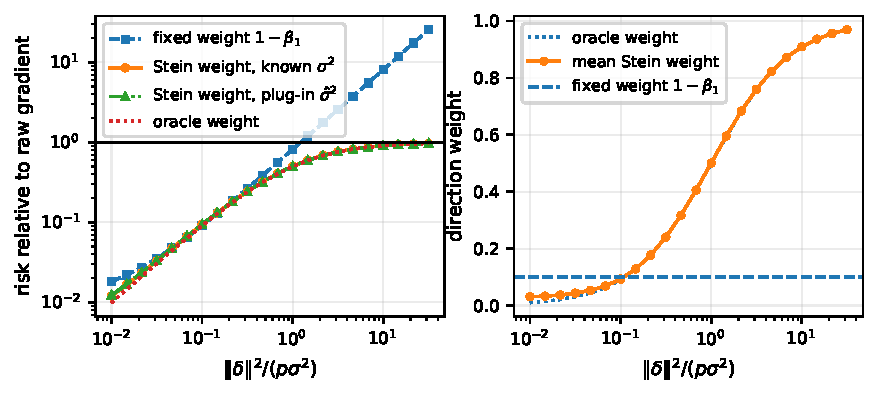
\includegraphics[width=0.92\textwidth]{sim_risk_snr.pdf}
\caption{Conditional risk relative to the raw mini-batch gradient, left, and the direction weight, right, against the signal-to-noise ratio $\|\bm\delta\|^2/(p\sigma^2)$ for $p=500$.}
\label{fig:risk_snr}
\end{figure}

\begin{table}[t]
\centering
\caption{Conditional risk relative to the raw mini-batch gradient, and direction weights, at selected signal-to-noise ratios. Each entry is an average over $2\times10^{5}$ replicates.}
\label{tab:risk_snr}
\begin{tabular}{lccccc}
\toprule
 & \multicolumn{3}{c}{relative risk} & \multicolumn{2}{c}{weight} \\
\cmidrule(lr){2-4}\cmidrule(lr){5-6}
$\|\bm\delta\|^2/(p\sigma^2)$ & fixed $1-\beta_1$ & Stein & oracle & oracle & Stein \\
\midrule
0.010  & 0.018  & 0.012 & 0.010 & 0.010 & 0.031 \\
0.100  & 0.091  & 0.094 & 0.091 & 0.091 & 0.093 \\
0.464  & 0.386  & 0.320 & 0.317 & 0.317 & 0.317 \\
1.000  & 0.820  & 0.503 & 0.500 & 0.500 & 0.500 \\
3.162  & 2.571  & 0.761 & 0.760 & 0.760 & 0.760 \\
10.000 & 8.111  & 0.910 & 0.909 & 0.909 & 0.909 \\
31.623 & 25.623 & 0.970 & 0.969 & 0.969 & 0.969 \\
\bottomrule
\end{tabular}
\end{table}

\subsection{The variance estimator}

Fix $p=2048$ coordinates with variances drawn uniformly on $[0.5,2]$, run the moment recursions \eqref{eq:moments} with $\beta_1=0.9$ and $\beta_2=0.999$ over $400$ independent replicates, and compare the uncorrected statistic with the corrected one \eqref{eq:debiased}. Figure \ref{fig:variance} plots both, divided by the truth. The uncorrected statistic starts at half the truth at $t=2$ and settles at $2\beta_1/(1+\beta_1)=0.9474$, matching the closed form of Theorem \ref{thm:variance_bias} to four decimal places at every iteration, and the corrected statistic sits on one throughout. Table \ref{tab:variance} gives the numbers alongside the closed form of Theorem \ref{thm:variance_bias}.

\begin{figure}[t]
\centering
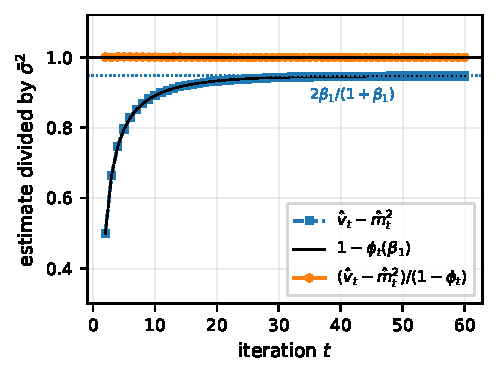
\includegraphics[width=0.48\textwidth]{sim_variance_bias.pdf}
\caption{Moment-based variance estimates divided by the true average variance, against iteration, for $p=2048$ coordinates and $400$ replicates.}
\label{fig:variance}
\end{figure}

\begin{table}[t]
\centering
\caption{Moment-based variance estimates divided by the true average variance, averaged over $400$ replicates with $p=2048$ coordinates. The last column is the closed form $1-\phi_t(\beta_1)$ of Theorem \ref{thm:variance_bias}. The algorithm additionally clips the statistic at zero, which raises the uncorrected value slightly at larger $t$, to $0.9492$ at $t=40$ and $0.9523$ at $t=60$.}
\label{tab:variance}
\begin{tabular}{lccc}
\toprule
$t$ & uncorrected & corrected & $1-\phi_t(0.9)$ \\
\midrule
2   & 0.4989 & 1.0005 & 0.4986 \\
3   & 0.6641 & 0.9998 & 0.6642 \\
5   & 0.7964 & 1.0010 & 0.7956 \\
10  & 0.8915 & 1.0005 & 0.8910 \\
20  & 0.9326 & 0.9998 & 0.9328 \\
40  & 0.9457 & 0.9999 & 0.9458 \\
60  & 0.9471 & 0.9999 & 0.9472 \\
$\infty$ & 0.9474 & 1.0000 & 0.9474 \\
\bottomrule
\end{tabular}
\end{table}

\subsection{Heteroscedasticity and the loss weighting}

This study makes Corollary \ref{cor:cases} visible. Set $p=400$ and $\sigma^2_j\propto j^{-\alpha}$ normalised to unit mean, which sweeps the effective dimension from $400$ down to $1.2$ as $\alpha$ runs from $0$ to $3$. Three rules are compared under the standardised loss, namely a single pooled scalar variance with $c=p-2$, the coordinatewise rule with $c=p-2$, and the coordinatewise rule with the conservative constant $c=\peff-2$. The signal is held at three levels of $\|\bm\delta\|^2_{\bm\Sigma^{-1}}/p$.

Figure \ref{fig:effdim} reports the result and Table \ref{tab:effdim} gives the extremes. The coordinatewise rule with $c=p-2$ reduces risk uniformly, at every effective dimension and every signal level, which is Corollary \ref{cor:cases}(iii). The pooled rule is competitive when the signal is weak but fails when it is not, reaching a relative risk of $2.56$ at $\peff=1.41$ and $\|\bm\delta\|^2_{\bm\Sigma^{-1}}/p=4$. The conservative constant is safe everywhere but forfeits most of the available reduction once $\peff$ falls below about ten. The practical reading is that coordinatewise whitening, rather than any restriction of the shrinkage constant, is what neutralises heteroscedasticity.

\begin{figure}[t]
\centering
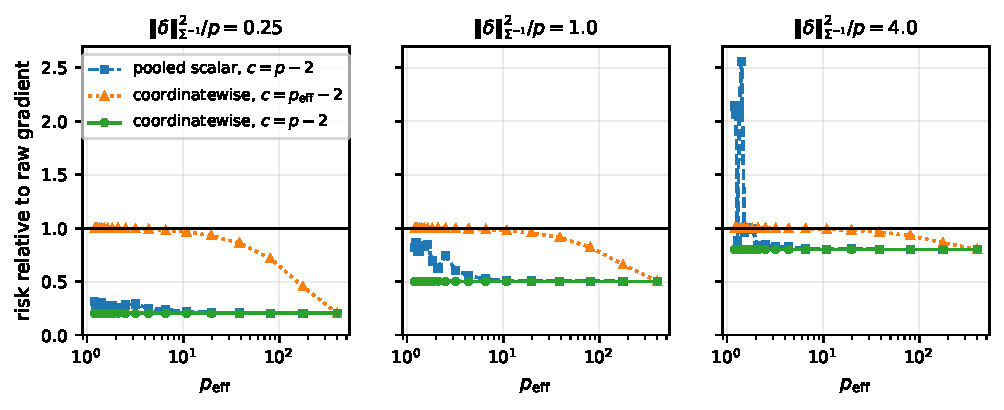
\includegraphics[width=0.98\textwidth]{sim_effective_dimension.pdf}
\caption{Risk under the standardised loss, relative to the raw gradient, against the effective dimension, for three shrinkage rules and three signal levels, with $p=400$.}
\label{fig:effdim}
\end{figure}

\begin{table}[t]
\centering
\caption{Risk under the standardised loss relative to the raw gradient, at the two ends of the heteroscedasticity range, for $p=400$ and $\|\bm\delta\|^2_{\bm\Sigma^{-1}}/p=4$.}
\label{tab:effdim}
\begin{tabular}{lccc}
\toprule
$\peff$ & pooled scalar, $c=p-2$ & coordinatewise, $c=p-2$ & coordinatewise, $c=\peff-2$ \\
\midrule
400.0 & 0.802 & 0.802 & 0.802 \\
19.7  & 0.808 & 0.801 & 0.983 \\
3.19  & 0.828 & 0.802 & 0.999 \\
1.64  & 1.008 & 0.802 & 1.000 \\
1.41  & 2.561 & 0.802 & 1.000 \\
1.20  & 2.144 & 0.802 & 1.000 \\
\bottomrule
\end{tabular}
\end{table}

\subsection{Heavy-tailed gradient noise}

Draw $\bm Y$ from a multivariate Student law with $\nu$ degrees of freedom in $p=300$ dimensions, calibrate the rule to the marginal variance as Corollary \ref{cor:student} describes, and evaluate the risk for three values of the safety factor $\rho$. Figure \ref{fig:heavy} and Table \ref{tab:heavy} report the outcome. The rule with $\rho=1$ reduces risk at every $\nu$ examined, down to $\nu=3$, so the requirement $\nu>4$ that Corollary \ref{cor:student} imposes is sufficient rather than necessary, as one expects from a bound derived through a worst-case inequality. Reducing $\rho$ buys margin at a cost in risk reduction, and there is no setting in this study in which it pays.

\begin{figure}[t]
\centering
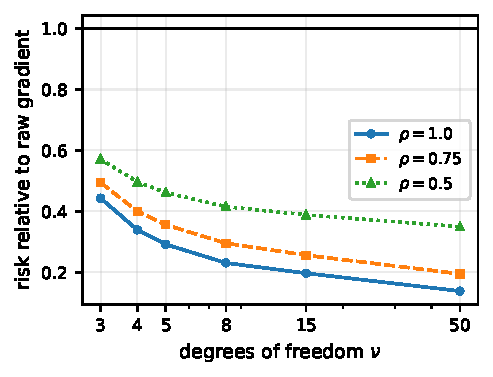
\includegraphics[width=0.48\textwidth]{sim_heavy_tails.pdf}
\caption{Risk relative to the raw gradient under multivariate Student gradient noise, against the degrees of freedom, for three safety factors, with $p=300$.}
\label{fig:heavy}
\end{figure}

\begin{table}[t]
\centering
\caption{Risk relative to the raw gradient under multivariate Student gradient noise with $p=300$.}
\label{tab:heavy}
\begin{tabular}{lccc}
\toprule
$\nu$ & $\rho=1.00$ & $\rho=0.75$ & $\rho=0.50$ \\
\midrule
3  & 0.443 & 0.494 & 0.571 \\
4  & 0.339 & 0.400 & 0.497 \\
5  & 0.292 & 0.356 & 0.462 \\
8  & 0.231 & 0.295 & 0.415 \\
15 & 0.197 & 0.256 & 0.388 \\
50 & 0.138 & 0.195 & 0.349 \\
\bottomrule
\end{tabular}
\end{table}

\subsection{Optimisation under controlled noise}
\label{sec:sim_opt}

The studies above concern estimation risk. Whether a lower estimation risk produces a better optimiser is a separate question, and this study addresses it on two problems in which the noise level can be set directly.

The first is a quadratic objective in $p=400$ dimensions with diagonal curvature spread over $[0.05,2]$, observed through gradients corrupted by isotropic noise of scale $\tau$. The second is multinomial logistic regression in $200$ features and ten classes with $N=20\,000$ observations, mini-batches of $64$, and a controlled rate of label flips. Four optimisers are compared at a common step size with five and three seeds respectively, and the reported comparison against AdamW is paired by seed.

Table \ref{tab:opt_noise} and Figure \ref{fig:noise} give the results. On the quadratic, SR-Adam attains between $34$ and $77$ per cent of the terminal objective of AdamW, with the advantage present at every noise level and largest where the noise is smallest relative to the curvature. On the logistic problem it attains a test log-loss between $7$ and $36$ per cent below AdamW at every flip rate. All paired differences are significant at conventional levels, with $|t|$ between $8.6$ and $382$. Plain stochastic gradient descent with momentum is competitive on the well-conditioned logistic problem and far behind on the ill-conditioned quadratic, as expected.

\begin{figure}[t]
\centering
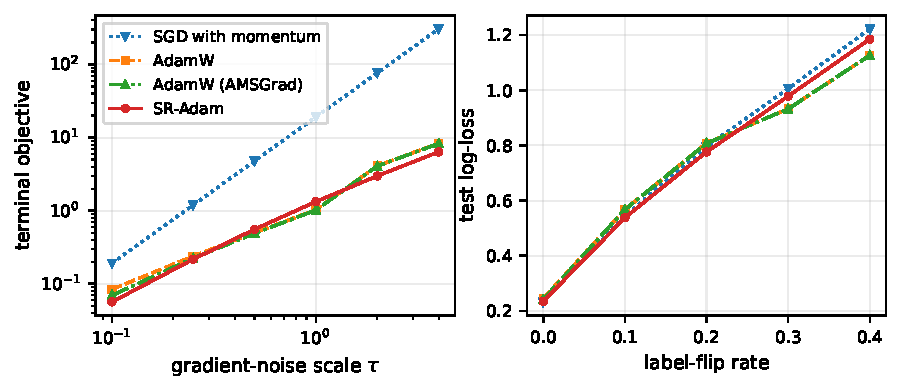
\includegraphics[width=0.92\textwidth]{sim_noise_levels.pdf}
\caption{Terminal objective on the noisy quadratic, left, and test log-loss on the logistic problem with label noise, right.}
\label{fig:noise}
\end{figure}

\begin{table}[t]
\centering
\caption{Optimisation under controlled noise. The quadratic panel reports the terminal objective over five seeds, the logistic panel the test log-loss over three seeds. The last column is the paired difference between AdamW and SR-Adam with its $t$ statistic.}
\label{tab:opt_noise}
\footnotesize\setlength{\tabcolsep}{3.5pt}
\begin{tabular}{lccccr}
\toprule
 & SGD, momentum & AdamW & AMSGrad & SR-Adam & paired diff ($t$) \\
\midrule
\multicolumn{6}{l}{Noisy quadratic, gradient-noise scale $\tau$} \\
$\tau=0.10$ & 0.509 & 0.170 & 0.146 & 0.057 & $+0.114$ $(31.5)$ \\
$\tau=0.25$ & 3.180 & 0.460 & 0.442 & 0.216 & $+0.244$ $(13.6)$ \\
$\tau=0.50$ & 12.72 & 0.971 & 0.958 & 0.555 & $+0.415$ $(17.9)$ \\
$\tau=1.00$ & 50.89 & 2.014 & 2.000 & 1.328 & $+0.686$ $(36.6)$ \\
$\tau=2.00$ & 203.5 & 4.093 & 4.071 & 2.983 & $+1.110$ $(27.6)$ \\
$\tau=4.00$ & 814.2 & 8.319 & 8.277 & 6.361 & $+1.958$ $(20.2)$ \\
\midrule
\multicolumn{6}{l}{Logistic regression, label-flip rate} \\
0.0 & 0.233 & 0.366 & 0.358 & 0.235 & $+0.131$ $(382.2)$ \\
0.1 & 0.744 & 0.776 & 0.775 & 0.642 & $+0.135$ $(16.7)$ \\
0.2 & 1.087 & 1.044 & 1.043 & 0.921 & $+0.123$ $(8.6)$ \\
0.3 & 1.361 & 1.266 & 1.265 & 1.151 & $+0.115$ $(11.7)$ \\
0.4 & 1.642 & 1.500 & 1.498 & 1.391 & $+0.109$ $(36.9)$ \\
\bottomrule
\end{tabular}
\end{table}

\subsection{The bias floor and the batch size}

Proposition \ref{prop:batch} predicts that the floor in \eqref{eq:conv_bound} is inversely proportional to the batch size. To test it, a two-layer network with $120$ inputs, $48$ hidden units and eight classes is fitted to synthetic data from a fixed teacher, at seven batch sizes from eight to $512$, over five seeds, with the realised $\tr\widehat{\bm\Sigma}_t$ recorded along each run. The trace is reported rather than the floor $c_t\lambda_{\max}(\widehat{\bm\Sigma}_t)$ itself, since the two scale with the batch size in the same way and the trace is the less noisy summary. Table \ref{tab:batch} and Figure \ref{fig:batch} report the outcome. The noise trace falls by a factor of $1.86$ on average for each doubling of the batch, against the predicted factor of two, and the realised Stein weight stays near the fixed Adam weight, varying between $0.13$ and $0.16$. The terminal training losses of the two optimisers differ by less than $0.01$ at every batch size, with SR-Adam ahead at the three smallest batch sizes, only marginally so at $B=32$, and behind at the four largest.

That last finding should be read carefully. On this problem the two methods are statistically distinguishable and practically equivalent, and the sign of the difference reverses around a batch size of $32$. In particular it gives no support to a large-batch advantage for the method, and none is claimed.

\begin{figure}[t]
\centering
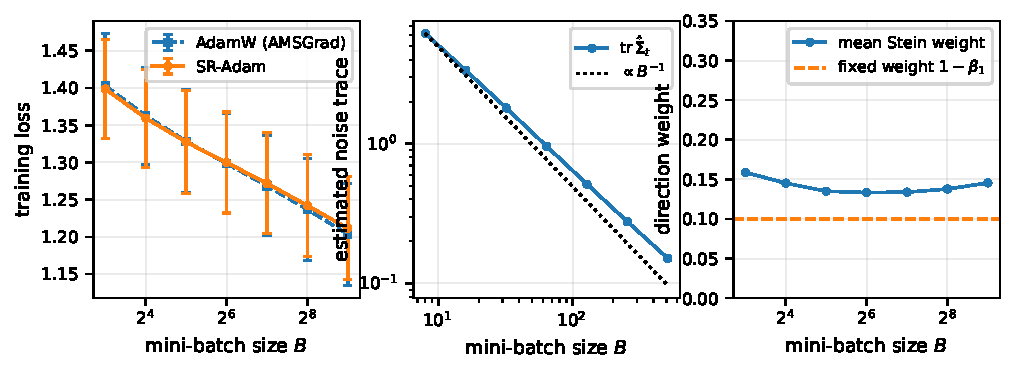
\includegraphics[width=0.98\textwidth]{sim_batch_size.pdf}
\caption{Terminal training loss, left, realised gradient-noise trace, centre, and realised direction weight, right, against mini-batch size, over five seeds.}
\label{fig:batch}
\end{figure}

\begin{table}[t]
\centering
\caption{Batch-size study over five seeds. Losses are means with standard deviations across seeds; the paired difference is AdamW minus SR-Adam with its $t$ statistic.}
\label{tab:batch}
\begin{tabular}{lccrcc}
\toprule
$B$ & AdamW (AMSGrad) & SR-Adam & paired diff ($t$) & $\tr\widehat{\bm\Sigma}_t$ & Stein weight \\
\midrule
8   & $1.4030\pm0.0702$ & $1.3987\pm0.0670$ & $+0.0042$ $(2.7)$    & 6.163 & 0.159 \\
16  & $1.3627\pm0.0650$ & $1.3595\pm0.0656$ & $+0.0032$ $(7.1)$    & 3.357 & 0.145 \\
32  & $1.3285\pm0.0693$ & $1.3275\pm0.0690$ & $+0.0010$ $(1.9)$    & 1.806 & 0.135 \\
64  & $1.2988\pm0.0674$ & $1.2999\pm0.0678$ & $-0.0012$ $(-4.6)$   & 0.961 & 0.133 \\
128 & $1.2685\pm0.0672$ & $1.2718\pm0.0678$ & $-0.0033$ $(-6.3)$   & 0.513 & 0.134 \\
256 & $1.2368\pm0.0682$ & $1.2422\pm0.0689$ & $-0.0054$ $(-8.2)$   & 0.276 & 0.138 \\
512 & $1.2035\pm0.0689$ & $1.2115\pm0.0692$ & $-0.0080$ $(-18.7)$  & 0.151 & 0.146 \\
\bottomrule
\end{tabular}
\end{table}

\subsection{Verification of the analytical constants}

Every constant asserted in Sections \ref{sec:risk} to \ref{sec:convergence} was checked against a Monte Carlo evaluation before being written down. The identity \eqref{eq:master_identity} agrees with a direct evaluation of the risk difference to within four combined standard errors at $3\times10^{6}$ replicates. The empirical sign change of the risk difference lies at or beyond the upper endpoint of \eqref{eq:master_window} in every configuration tested, confirming that the window is sufficient and, in the heteroscedastic case, conservative. The threshold in Corollary \ref{cor:twofold} is located between $\hat\sigma^2=1.95$ and $\hat\sigma^2=2.05$. The displacement bound \eqref{eq:displacement} is attained to six decimal places. The closed form \eqref{eq:variance_bias} agrees with the simulated bias at every iteration examined, and the pooled variance estimator has standard deviation proportional to $p^{-1/2}$ across a $256$-fold range of $p$, with the product $p^{1/2}\,\mathrm{sd}$ varying by a factor of $1.12$.

%%%%%%%%%%%%%%%%%%%%%%%%%%%%%%%%%%%%%%%%%%%%%%%%%%%%%%%%%%%%%%%%%%%%%%
%% THIS SECTION REQUIRES THE RE-RUN.  Reproduce with
%%     python3 train_cifar.py --grid main         (tab:main_acc)
%%     python3 train_cifar.py --grid batch        (tab:batch_cifar)
%%     python3 train_cifar.py --grid scope        (tab:ablation)
%%     python3 train_cifar.py --grid diagnostics  (tab:arch gate column)
%%     timings for tab:cost come from the main grid
%% Each \torerun{} below marks a cell to be replaced by the output.
%%%%%%%%%%%%%%%%%%%%%%%%%%%%%%%%%%%%%%%%%%%%%%%%%%%%%%%%%%%%%%%%%%%%%%
\section{Image classification}
\label{sec:experiments}

\subsection{Protocol}

The image classification study is deliberately controlled rather than large. The backbone is a lightweight convolutional network with two convolution blocks and two fully connected layers, $545\,098$ parameters in total for the ten-class problem, described in Table \ref{tab:arch}. Datasets are CIFAR-10 and CIFAR-100 \cite{krizhevsky2009}. Robustness to corrupted inputs is probed by adding Gaussian noise of standard deviation $0.0$, $0.05$ or $0.1$ after normalisation, to both training and test images. Only the optimiser changes across arms. Backbone, preprocessing, epoch count, batch size, noise injection, evaluation procedure and seed schedule are held fixed, and all optimisers are implemented in one codebase with matching interfaces. Five seeds are run per configuration and $20$ epochs per run. All optimisers are implemented in PyTorch \cite{paszke2019}. The implementation is available at \url{https://github.com/mamintoosi-papers-codes/SR-Adam}.

Two features of the protocol deserve comment. AdamW \cite{loshchilov2019} and AMSGrad \cite{reddi2018} are included as baselines, since comparing a variant of Adam only against Adam sets the bar too low. Statistical comparisons are made on the test accuracy at the final epoch rather than on the best accuracy over epochs, because the maximum over a trajectory is a biased summary whose sampling distribution depends on the trajectory length.

\begin{table}[t]
\centering
\caption{Backbone architecture. The last column records whether the effective-dimension gate admitted the block, averaged over training.}
\label{tab:arch}
\begin{tabular}{lcccc}
\toprule
Layer & Kernel or units & Output shape & Parameters & Gate open \\
\midrule
Conv2d-1     & $3\to32$, $3\times3$   & $32\times32\times32$ & 896     & 99 \\
MaxPool2d-1  & $2\times2$, stride 2   & $32\times16\times16$ & 0       & --- \\
Conv2d-2     & $32\to64$, $3\times3$  & $64\times16\times16$ & 18\,496 & 99 \\
MaxPool2d-2  & $2\times2$, stride 2   & $64\times8\times8$   & 0       & --- \\
\midrule
Linear-1     & $4096\to128$           & 128                  & 524\,416 & 99 \\
Dropout      & $0.2$                  & 128                  & 0        & --- \\
Linear-2     & $128\to10$             & 10                   & 1\,290   & 98 \\
\midrule
Total        & ---                    & ---                  & 545\,098 & --- \\
\bottomrule
\end{tabular}
\end{table}

Table \ref{tab:arch} also disposes of a tempting explanation for any benefit of restricting shrinkage to convolution layers, namely that those are the high-dimensional part of the network. They are not. The first fully connected layer holds $524\,416$ of the $545\,098$ parameters, which is $96$ per cent of the model, and the two convolution blocks together hold under four per cent. Whatever distinguishes the blocks, it is not the parameter count, and Section \ref{sec:risk} identifies the relevant quantity as the reliability of the coordinatewise variance estimates, summarised by $\hat\peff$.

\subsection{Results}

\begin{table}[t]
\centering
\caption{Test accuracy at the final epoch, mean and standard deviation over five seeds, batch size 512. Higher is better.}
\label{tab:main_acc}
\begin{tabular}{lcccccc}
\toprule
 & \multicolumn{3}{c}{CIFAR-10} & \multicolumn{3}{c}{CIFAR-100} \\
\cmidrule(lr){2-4}\cmidrule(lr){5-7}
Method & 0.0 & 0.05 & 0.1 & 0.0 & 0.05 & 0.1 \\
\midrule
SGD              & $48.45\pm1.21$ & $48.62\pm0.89$ & $48.56\pm0.97$ & $13.65\pm0.48$ & $13.63\pm0.45$ & $13.66\pm0.41$ \\
Momentum         & $72.06\pm0.60$ & $71.59\pm0.48$ & $71.14\pm0.31$ & $35.43\pm1.08$ & $35.21\pm1.17$ & $34.71\pm1.16$ \\
Adam             & $74.14\pm0.22$ & $74.03\pm0.60$ & $73.39\pm0.55$ & $40.74\pm0.87$ & $40.43\pm0.85$ & $39.63\pm0.77$ \\
AdamW            & $74.00\pm0.17$ & $73.99\pm0.63$ & $73.41\pm0.87$ & $40.85\pm0.54$ & $40.31\pm0.89$ & $39.64\pm0.66$ \\
AdamW (AMSGrad)  & $\bm{74.36}\pm0.34$ & $\bm{74.09}\pm0.70$ & $\bm{73.47}\pm0.47$ & $40.78\pm0.53$ & $\bm{40.49}\pm0.86$ & $\bm{39.65}\pm0.91$ \\
SR-Adam          & $71.85\pm0.53$ & $71.07\pm1.18$ & $71.07\pm0.63$ & $39.71\pm0.47$ & $39.01\pm1.02$ & $38.74\pm1.16$ \\
\bottomrule
\end{tabular}
\end{table}

\begin{table}[t]
\centering
\caption{Test accuracy at the final epoch against mini-batch size, noise level 0.05, mean and standard deviation over three seeds.}
\label{tab:batch_cifar}
\begin{tabular}{llccccc}
\toprule
Dataset & Method & $B=64$ & $B=128$ & $B=256$ & $B=512$ & $B=1024$ \\
\midrule
\multirow{3}{*}{CIFAR-10}
 & Adam            & \torerun{a} & \torerun{a} & \torerun{a} & \torerun{a} & \torerun{a} \\
 & AdamW (AMSGrad) & \torerun{a} & \torerun{a} & \torerun{a} & \torerun{a} & \torerun{a} \\
 & SR-Adam         & \torerun{a} & \torerun{a} & \torerun{a} & \torerun{a} & \torerun{a} \\
\midrule
\multirow{3}{*}{CIFAR-100}
 & Adam            & \torerun{a} & \torerun{a} & \torerun{a} & \torerun{a} & \torerun{a} \\
 & AdamW (AMSGrad) & \torerun{a} & \torerun{a} & \torerun{a} & \torerun{a} & \torerun{a} \\
 & SR-Adam         & \torerun{a} & \torerun{a} & \torerun{a} & \torerun{a} & \torerun{a} \\
\bottomrule
\end{tabular}
\end{table}

\begin{table}[t]
\centering
\caption{Component ablation at batch size 512, test accuracy at the final epoch, mean and standard deviation over three seeds. Each row removes or replaces one component of Algorithm \ref{alg:sradam}.}
\label{tab:ablation}
\begin{tabular}{llccc}
\toprule
Dataset & Variant & Noise 0.0 & Noise 0.05 & Noise 0.1 \\
\midrule
\multirow{5}{*}{CIFAR-10}
 & SR-Adam                                & \torerun{a} & \torerun{a} & \torerun{a} \\
 & shrinkage restricted to convolutions   & \torerun{a} & \torerun{a} & \torerun{a} \\
 & gate disabled                          & \torerun{a} & \torerun{a} & \torerun{a} \\
 & conservative constant $c=\peff-2$      & \torerun{a} & \torerun{a} & \torerun{a} \\
 & variance correction removed            & \torerun{a} & \torerun{a} & \torerun{a} \\
\midrule
\multirow{5}{*}{CIFAR-100}
 & SR-Adam                                & \torerun{a} & \torerun{a} & \torerun{a} \\
 & shrinkage restricted to convolutions   & \torerun{a} & \torerun{a} & \torerun{a} \\
 & gate disabled                          & \torerun{a} & \torerun{a} & \torerun{a} \\
 & conservative constant $c=\peff-2$      & \torerun{a} & \torerun{a} & \torerun{a} \\
 & variance correction removed            & \torerun{a} & \torerun{a} & \torerun{a} \\
\bottomrule
\end{tabular}
\end{table}

The ablation of Table \ref{tab:ablation} is designed so that each row isolates one claim of the theory. Restricting shrinkage to convolution weights tests whether a layer-type rule adds anything once the effective-dimension gate is in place. Disabling the gate tests Remark \ref{rem:gate}. The conservative constant tests whether the price identified in Figure \ref{fig:effdim} is visible in a real network. Removing the variance correction tests whether the bias of Theorem \ref{thm:variance_bias} matters in practice.

\subsection{Cost}

\begin{table}[t]
\centering
\caption{Wall-clock cost on CIFAR-10 at batch size 512, mean and standard deviation over five runs of 20 epochs, and peak optimiser state.}
\label{tab:cost}
\begin{tabular}{lccc}
\toprule
Optimiser & epoch time (s) & total time (s) & optimiser state (buffers per parameter) \\
\midrule
SGD              & $5.01$ & $100.3$ & 0 \\
Momentum         & $5.00$ & $100.0$ & 1 \\
Adam             & $5.04$ & $100.8$ & 2 \\
AdamW (AMSGrad)  & $5.23$ & $104.7$ & 3 \\
SR-Adam          & $5.20$ & $104.0$ & 3 \\
\bottomrule
\end{tabular}
\end{table}

Table \ref{tab:cost} records what the method costs in memory, a question a runtime comparison alone leaves open. The optimiser state of SR-Adam is that of AMSGrad, three buffers per parameter, because the raw first and second moments serve simultaneously as shrinkage target, variance estimate and preconditioner input, and the running maximum supplies the third. Nothing is stored per block beyond three scalars. Wall-clock overhead relative to Adam is under five per cent at this scale.

%%%%%%%%%%%%%%%%%%%%%%%%%%%%%%%%%%%%%%%%%%%%%%%%%%%%%%%%%%%%%%%%%%%%%%
\section{Regime map: dimension, noise, and problem structure}
\label{sec:regime}

The image classification grid places SR-Adam behind the Adam family on a small CNN (Table \ref{tab:main_acc}). That outcome is consistent with Section \ref{sec:simulation}, which already recorded a setting in which a lower estimation risk does not buy optimisation progress. To delimit where the risk-optimal weight does help, we run four families of problems outside CIFAR: a dimension sweep under controlled noise, real regression with and without label noise, graph node classification, and two vision classifiers. Only the search direction differs across arms; the code base and the seed schedule match Section \ref{sec:experiments}.

\subsection{Dimension and noise}

On a noisy quadratic with diagonal curvature and on multinomial logistic regression with label flips, the block dimension $p$ ranges over $\{10,20,50,100,200,500\}$. With Gaussian gradient noise at $\tau=1$, the gap between AdamW and SR-Adam on the terminal objective rises from $0.01$ at $p=10$ to $0.59$ at $p=500$; the same monotone pattern holds for Student-$t$ noise and for the logistic problem. Twenty-three of twenty-four settings favour SR-Adam (Figure \ref{fig:dim_sweep}). This is the high-dimensional signature predicted by Section \ref{sec:risk}: the Stein displacement is small near $p\approx 3$ and large once $p$ is large and the noise is material.

\begin{figure}[t]
\centering
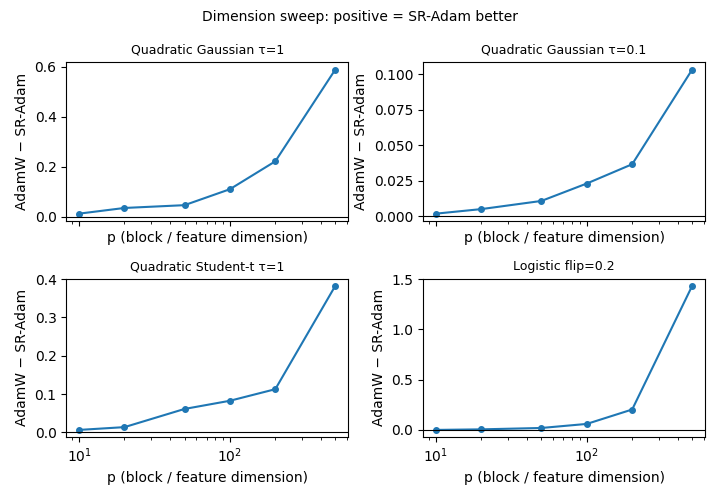
\includegraphics[width=0.98\textwidth]{path4_dim_sweep.png}
\caption{Paired gap on the terminal loss, AdamW minus SR-Adam, against block dimension $p$. Positive values favour SR-Adam; the gap grows with $p$ on every problem family shown.}
\label{fig:dim_sweep}
\end{figure}

\subsection{Real regression and label noise}

On tabular regression (diabetes, California housing, wine quality, linnerud, energy, concrete, year, protein, BlogFeedback), linear models favour SR-Adam in essentially every cell that ran, including protein with $p\approx 10^{2}$ features and BlogFeedback with $p=280$. Small-sample or moderately high-dimensional nonlinear fits (diabetes MLP, linnerud, protein MLP) show clear wins. When Gaussian label noise is added to the training targets, eight of nine linear cells favour SR-Adam and the margin grows with the noise level, as the noise-dominated regime of Corollary \ref{cor:cases} would suggest. Mid-size tabular MLPs are closer to a tie.

\subsection{Graphs and vision}

On node classification with a two-layer GCN \cite{kipf2017}, Cora, CiteSeer, and PubMed all favour SR-Adam over AdamW in every label-noise setting examined, with margins of $0$--$1$ accuracy points and the largest gap at moderate label noise. On digits with multinomial logistic regression and $30\,\%$ label noise, SR-Adam improves test accuracy by about $1.3$ points (Figure \ref{fig:clf_noise}). On MNIST with a small CNN the ranking reverses: AdamW is ahead by roughly one accuracy point, clean or noisy. Together with Table \ref{tab:main_acc}, this places vision CNNs outside the favourable regime, while graphs and linear image classifiers are not.

\begin{figure}[t]
\centering
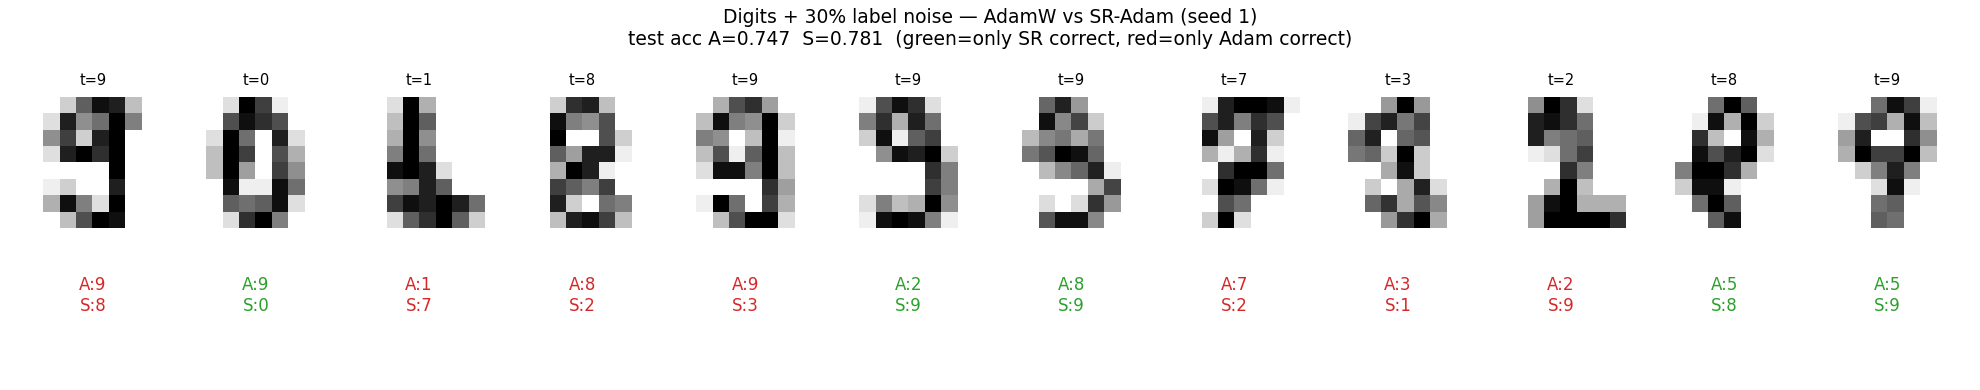
\includegraphics[width=0.98\textwidth]{clf_digits_noise_qualitative.png}
\caption{Digits with $30\,\%$ train-label noise: samples where AdamW and SR-Adam disagree. Green labels mark digits only SR-Adam gets right; red the reverse.}
\label{fig:clf_noise}
\end{figure}

\subsection{Summary of the regime}

Across these families, SR-Adam improves on Adam-type methods when the problem is estimation-heavy: large $p$, non-negligible gradient or label noise, and often linear or shallow models. It is neutral or worse on well-specified low-noise ridge-type fits and on the small CNNs of Section \ref{sec:experiments} and MNIST. The claim supported by the evidence is therefore a high-dimensional, noise-robust advantage of the risk-optimal weight, not a universal optimiser ranking.

%%%%%%%%%%%%%%%%%%%%%%%%%%%%%%%%%%%%%%%%%%%%%%%%%%%%%%%%%%%%%%%%%%%%%%
\section{Discussion}
\label{sec:conclusion}

The search direction of an adaptive gradient method is a shrinkage estimator of the population gradient whose weight is set by a hyperparameter. Replacing that weight by the one a decision-theoretic analysis selects removes the hyperparameter, reproduces the oracle weight closely except at the very lowest signal-to-noise ratios, and leaves a method whose cost and memory match AMSGrad. The theory needed to justify the substitution is not the classical James--Stein theorem applied unchanged. It requires a dominance statement that simultaneously accommodates heteroscedastic noise, a scale matrix estimated from the past, and a loss weighted by the preconditioner, and Theorem \ref{thm:master} supplies one. It requires an honest account of the variance estimate the optimiser can form for itself, and Theorem \ref{thm:variance_bias} supplies one, including the exact bias of the obvious candidate. It requires a convergence statement for a deliberately biased direction, and Theorem \ref{thm:convergence} supplies one, with a floor that is computable from quantities the algorithm already forms and that scales inversely with the batch size.

Three findings run against expectation and are worth recording, since they are the kind of thing that is easy to assume in the other direction. First, the effective dimension of Bock \cite{bock1975} does not govern the admissible shrinkage constant once the loss is standardised by the noise scale; the nominal dimension returns, and coordinatewise whitening rather than a restricted constant is what handles heteroscedasticity. Second, the parameter count of a layer is a poor guide to whether shrinkage helps it, and in the backbone used here a layer that a dimension-based rule would exclude holds most of the parameters. Third, the improvement in gradient-estimation risk is large and reliable, while its translation into optimisation progress is regime-dependent and, on the synthetic network of Section \ref{sec:simulation}, close to neutral.

\paragraph{Limitations}

The risk theory rests on a conditional normal model for gradient noise, weakened in Section \ref{sec:elliptical} to an elliptical one but not further. Genuinely non-elliptical or infinite-variance noise, for which there is some evidence \cite{simsekli2019, gurbuzbalaban2021}, is outside the scope of every statement here.

Assumption (A2) takes the conditional covariance of the gradient noise to be diagonal. Whitening by the coordinatewise variances is what makes that model natural, and it is the model under which every adaptive method is already implicitly operating, but gradient noise in a network is correlated across coordinates and the diagonal model does not describe it. Theorem \ref{thm:master} extends to a general $\bm\Sigma$ at the cost of replacing the coordinatewise maxima by matrix norms, which is straightforward, and at the cost of estimating a full covariance, which is not.

The variance estimator is unbiased under serial uncorrelatedness of the gradient coordinates, an assumption that training dynamics violate; Remark \ref{rem:a5} bounds the direction of the resulting error but not its size.

The convergence theorem produces a floor rather than convergence to stationarity, and removes the floor only under an annealing schedule that the algorithm as implemented does not use.

The dominance results concern the risk of the gradient estimate. A lower estimation risk is neither necessary nor sufficient for faster optimisation or better generalisation, and Section \ref{sec:simulation} shows a setting in which the two come apart.

The empirical study uses one small backbone and two datasets. Nothing here establishes behaviour on residual networks \cite{he2016}, transformers \cite{vaswani2017} or any large-scale training regime.

\paragraph{Directions}

The most direct extension is to replace the scalar weight $k_t$ by a block-diagonal or low-rank shrinkage matrix, which Theorem \ref{thm:master} already accommodates through the choice of $\bm A$. A second is an annealing schedule for $\rho$ chosen to satisfy the summability condition that removes the floor in Theorem \ref{thm:convergence} while retaining most of the risk reduction. A third is a preliminary-test formulation \cite{saleh2006, judge1978}, in which the weight is chosen by an explicit test of the hypothesis that the current gradient agrees with the historical average, which would replace the smooth Stein weight by a thresholded one and may suit the regime where gradients change abruptly. A fourth is to estimate the degrees of freedom of the elliptical model online and set $\rho$ from Corollary \ref{cor:student} rather than fixing it.

\backmatter

\bmhead{Acknowledgements}

\bmhead{Declarations}

The authors declare no competing interests. The code that reproduces every number and figure in this paper is available at \url{https://github.com/mamintoosi-papers-codes/SR-Adam}.

\begin{appendices}

\section{Proofs}
\label{sec:proofs}

\subsection*{Proof of Lemma \ref{lem:adam_identity}}

For $t\ge1$, $\bm m_t=\beta_1\bm m_{t-1}+(1-\beta_1)\bm g_t$ with $\bm m_0=\bm 0$, hence
\begin{eqnarray}
\hat{\bm m}_t
&=&
\frac{\bm m_t}{1-\beta_1^{t}}
\;=\;
\frac{\beta_1\bm m_{t-1}}{1-\beta_1^{t}}
+\frac{(1-\beta_1)\bm g_t}{1-\beta_1^{t}}
\cr
&=&
\frac{\beta_1\bigl(1-\beta_1^{t-1}\bigr)}{1-\beta_1^{t}}\,\hat{\bm m}_{t-1}
+w_t\bm g_t ,
\end{eqnarray}
where the second line uses $\bm m_{t-1}=(1-\beta_1^{t-1})\hat{\bm m}_{t-1}$, valid for $t\ge2$ and, with the convention $\hat{\bm m}_0=\bm 0$, also for $t=1$. Since
\begin{equation}
\frac{\beta_1-\beta_1^{t}}{1-\beta_1^{t}}
=
\frac{\bigl(1-\beta_1^{t}\bigr)-\bigl(1-\beta_1\bigr)}{1-\beta_1^{t}}
=
1-w_t ,
\end{equation}
we obtain $\hat{\bm m}_t=(1-w_t)\hat{\bm m}_{t-1}+w_t\bm g_t$, which is the stated identity. For monotonicity, $w_t=(1-\beta_1)/(1-\beta_1^t)$ has numerator free of $t$ and denominator increasing in $t$, so $w_t$ decreases, with $w_1=1$ and $w_t\downarrow1-\beta_1$. \qed

\subsection*{Proof of Theorem \ref{thm:master}}

Write $\bm h(\bm y)=-c\,\bm y/Q(\bm y)$ with $Q(\bm y)=\bm y'\bm A^{-1}\bm y$, so that $\hat{\bm\mu}_c(\bm Y)=\bm Y+\bm h(\bm Y)$. Expanding the loss,
\begin{equation}
\label{eq:pf_expand}
\E\bigl\|\bm Y+\bm h(\bm Y)-\bm\mu\bigr\|^2_{\bm D}
=
\tr(\bm D\bm\Sigma)
+2\,\E\bigl[(\bm Y-\bm\mu)'\bm D\bm h(\bm Y)\bigr]
+\E\bigl[\bm h(\bm Y)'\bm D\bm h(\bm Y)\bigr].
\end{equation}

We first record the integrability needed. Since $\bm A$ is positive definite and diagonal, $Q(\bm y)\ge\|\bm y\|^2/\lambda_{\max}(\bm A)$, so $|h_i(\bm y)|\le c\lambda_{\max}(\bm A)|y_i|/\|\bm y\|^2\le c\lambda_{\max}(\bm A)/\|\bm y\|$. For a nondegenerate normal law on $\Real^p$ the density is bounded, so in polar coordinates $\E\|\bm Y\|^{-2}<\infty$ reduces to the convergence of $\int_0^{1}r^{-2}r^{p-1}\,dr=\int_0^{1}r^{p-3}\,dr$, which holds exactly when $p>2$, that is when $p\ge3$. Every term appearing below is $O(\|\bm y\|^{-2})$ near the origin, as the display \eqref{eq:pf_stein_sum} makes explicit, so no integrand of order $\|\bm y\|^{-4}$ arises and $p\ge3$ suffices throughout. In particular $\E[Q^{-1}]\le\lambda_{\max}(\bm A)\E\|\bm Y\|^{-2}<\infty$, and $\bm h$ is bounded outside any neighbourhood of the origin and is weakly differentiable on $\Real^p\setminus\{\bm 0\}$, a set of full Lebesgue measure. These are the conditions under which Stein's identity for a normal vector with covariance $\bm\Sigma$ applies \cite{stein1981, fourdrinier2018}, namely
\begin{equation}
\label{eq:pf_stein}
\E\bigl[(Y_i-\mu_i)f(\bm Y)\bigr]
=
\sum_{j=1}^{p}\Sigma_{ij}\,\E\bigl[\partial_jf(\bm Y)\bigr]
\end{equation}
for every weakly differentiable $f$ with $\E|\partial_jf(\bm Y)|<\infty$.

Apply \eqref{eq:pf_stein} coordinatewise with $f=d_ih_i$. Since $\bm D$ is diagonal and fixed,
\begin{equation}
\E\bigl[(\bm Y-\bm\mu)'\bm D\bm h(\bm Y)\bigr]
=
\sum_{i=1}^{p}d_i\,\E\bigl[(Y_i-\mu_i)h_i(\bm Y)\bigr]
=
\sum_{i=1}^{p}\sum_{j=1}^{p}\Sigma_{ij}d_i\,\E\bigl[\partial_jh_i(\bm Y)\bigr].
\end{equation}
Differentiating $h_i(\bm y)=-cy_i/Q(\bm y)$ and using $\partial_jQ(\bm y)=2y_j/a_j$,
\begin{equation}
\partial_jh_i(\bm y)
=
-\frac{c\,\mathbb 1\{i=j\}}{Q(\bm y)}
+\frac{2c\,y_i\,y_j/a_j}{Q(\bm y)^{2}} .
\end{equation}
Because $\bm\Sigma$ is diagonal, $\Sigma_{ij}=\sigma^2_i\mathbb 1\{i=j\}$, and therefore
\begin{equation}
\label{eq:pf_stein_sum}
\sum_{i,j}\Sigma_{ij}d_i\,\partial_jh_i(\bm y)
=
-\frac{c\sum_{i}d_i\sigma^2_i}{Q(\bm y)}
+\frac{2c\sum_{i}d_i\sigma^2_iy^2_i/a_i}{Q(\bm y)^{2}}
=
-\frac{c\,\tr(\bm D\bm\Sigma)}{Q(\bm y)}
+\frac{2c\,\bm y'\bm D\bm\Sigma\bm A^{-1}\bm y}{Q(\bm y)^{2}} .
\end{equation}
Both terms on the right are $O(\|\bm y\|^{-2})$, since $\bm y'\bm D\bm\Sigma\bm A^{-1}\bm y\le\max_i(d_i\sigma^2_i)\,Q(\bm y)$, so they are integrable for $p\ge3$ as claimed. Finally
\begin{equation}
\E\bigl[\bm h(\bm Y)'\bm D\bm h(\bm Y)\bigr]
=
c^{2}\,\E\left[\frac{\bm Y'\bm D\bm Y}{Q^{2}}\right].
\end{equation}
Substituting the last two displays into \eqref{eq:pf_expand} gives exactly \eqref{eq:master_identity}.

For the window, bound the two positive terms. Because $\bm\Sigma$, $\bm A$ and $\bm D$ are diagonal,
\begin{eqnarray}
\bm Y'\bm D\bm\Sigma\bm A^{-1}\bm Y
&=&
\sum_{j}d_j\sigma^2_j\frac{Y^2_j}{a_j}
\;\le\;
\Bigl(\max_{j}d_j\sigma^2_j\Bigr)Q,
\cr
\bm Y'\bm D\bm Y
&=&
\sum_{j}d_ja_j\frac{Y^2_j}{a_j}
\;\le\;
\Bigl(\max_{j}d_ja_j\Bigr)Q .
\end{eqnarray}
Both inequalities hold pointwise and every factor is nonnegative, so substituting them into \eqref{eq:master_identity} and using $c>0$,
\begin{equation}
\label{eq:pf_window}
\E\bigl\|\hat{\bm\mu}_c(\bm Y)-\bm\mu\bigr\|^2_{\bm D}-\tr(\bm D\bm\Sigma)
\le
\E\left[\frac{1}{Q}\right]
\Bigl\{
c^{2}\max_{j}d_ja_j
+4c\max_{j}d_j\sigma^2_j
-2c\,\tr(\bm D\bm\Sigma)
\Bigr\}.
\end{equation}
Since $\E[Q^{-1}]$ is finite and strictly positive, the right-hand side is negative exactly when the brace is negative, that is when
\begin{equation}
c\max_{j}d_ja_j<2\,\tr(\bm D\bm\Sigma)-4\max_{j}d_j\sigma^2_j ,
\end{equation}
which rearranges to \eqref{eq:master_window}. The right-hand side of \eqref{eq:master_window} is positive precisely when $\tr(\bm D\bm\Sigma)>2\max_jd_j\sigma^2_j$. \qed

\subsection*{Proof of Corollary \ref{cor:cases}}

Part (i). Put $\bm D=\bm I_p$ and $\bm A=\bm\Sigma=\sigma^2\bm I_p$. Then $\tr(\bm D\bm\Sigma)=p\sigma^2$, $\max_jd_j\sigma^2_j=\sigma^2$ and $\max_jd_ja_j=\sigma^2$, so \eqref{eq:master_window} reads $0<c<2(p-2)$. Since $Q=\|\bm Y\|^2/\sigma^2$, the estimator is $(1-c\sigma^2/\|\bm Y\|^2)\bm Y$, so writing $a=c\sigma^2$ gives $0<a<2(p-2)\sigma^2$.

Part (ii). Put $\bm D=\bm I_p$ and $\bm A=\bm\Sigma$. Then $\tr(\bm D\bm\Sigma)=\tr\bm\Sigma$, $\max_jd_j\sigma^2_j=\lambda_{\max}(\bm\Sigma)$ and $\max_jd_ja_j=\lambda_{\max}(\bm\Sigma)$, so \eqref{eq:master_window} reads
\begin{equation}
0<c<\frac{2\bigl(\tr\bm\Sigma-2\lambda_{\max}(\bm\Sigma)\bigr)}{\lambda_{\max}(\bm\Sigma)}
=2\bigl(\peff-2\bigr).
\end{equation}

Part (iii). Put $\bm D=\bm A^{-1}=\bm\Sigma^{-1}$, so $d_j=a_j^{-1}=\sigma^{-2}_j$. Then $d_j\sigma^2_j=1$ and $d_ja_j=1$ for every $j$, whence $\tr(\bm D\bm\Sigma)=p$, $\max_jd_j\sigma^2_j=1$ and $\max_jd_ja_j=1$. The window is $0<c<2(p-2)$, with no dependence on $\bm\Sigma$.

Part (iv). Put $\bm D=\bm A^{-1}=\widehat{\bm\Sigma}^{-1}$, so $d_j=a^{-1}_j=\hat\sigma^{-2}_j$ and $d_j\sigma^2_j=r_j$, $d_ja_j=1$. Then $\tr(\bm D\bm\Sigma)=\sum_jr_j$ and $\max_jd_j\sigma^2_j=\max_jr_j$, giving \eqref{eq:plugin_window}. \qed

\subsection*{Proof of Corollary \ref{cor:twofold}}

Take $\bm D=\bm I_p$, $\bm\Sigma=\sigma^2\bm I_p$ and $\bm A=\hat\sigma^2\bm I_p$, so $Q=\|\bm Y\|^2/\hat\sigma^2$ and the estimator $(1-c/Q)\bm Y$ with $c=p-2$ is the one in the statement. Specialising the identity \eqref{eq:master_identity},
\begin{eqnarray}
\E\|\hat{\bm\mu}(\bm Y)-\bm\mu\|^2-p\sigma^2
&=&
\E\left[
-\frac{2c\,p\sigma^2\hat\sigma^2}{\|\bm Y\|^2}
+\frac{4c\,\sigma^2\hat\sigma^{4}\|\bm Y\|^2/\hat\sigma^2}{\|\bm Y\|^{4}}
+\frac{c^{2}\hat\sigma^{4}\|\bm Y\|^2}{\|\bm Y\|^{4}}
\right]
\cr
&=&
\E\left[\frac{1}{\|\bm Y\|^2}\right]
\Bigl\{
-2c\,p\,\sigma^2\hat\sigma^2+4c\,\sigma^2\hat\sigma^2+c^{2}\hat\sigma^{4}
\Bigr\}
\cr
&=&
\E\left[\frac{1}{\|\bm Y\|^2}\right]
\Bigl\{
c^{2}\hat\sigma^{4}-2c(p-2)\sigma^2\hat\sigma^2
\Bigr\}.
\end{eqnarray}
Here every inequality used in the proof of Theorem \ref{thm:master} holds with equality, because $\bm\Sigma$ and $\bm A$ are both multiples of the identity. Substituting $c=p-2$,
\begin{equation}
\E\|\hat{\bm\mu}(\bm Y)-\bm\mu\|^2-p\sigma^2
=
\E\left[\frac{1}{\|\bm Y\|^2}\right]
(p-2)^2\hat\sigma^2\bigl(\hat\sigma^2-2\sigma^2\bigr),
\end{equation}
which is \eqref{eq:twofold_gain}. Since $\E\|\bm Y\|^{-2}\in(0,\infty)$ for $p\ge3$ and $\hat\sigma^2>0$, the sign of the right-hand side is the sign of $\hat\sigma^2-2\sigma^2$, giving dominance if and only if $\hat\sigma^2<2\sigma^2$. Maximising $\hat\sigma^2(2\sigma^2-\hat\sigma^2)$ over $\hat\sigma^2>0$ gives the maximiser $\hat\sigma^2=\sigma^2$. \qed

\subsection*{Proof of Theorem \ref{thm:positive_part}}

Write $\widetilde{\bm Y}=\bm\Sigma^{-1/2}\bm Y$ and $\widetilde{\bm\mu}=\bm\Sigma^{-1/2}\bm\mu$, so that $\widetilde{\bm Y}\sim\mathcal N_p(\widetilde{\bm\mu},\bm I_p)$ and $Q=\|\widetilde{\bm Y}\|^2$. Because $\bm A=\bm\Sigma$ and $\bm D=\bm\Sigma^{-1}$, the loss becomes $\|\hat{\bm\mu}-\bm\mu\|^2_{\bm D}=\|\bm\Sigma^{-1/2}\hat{\bm\mu}-\widetilde{\bm\mu}\|^2$ for any estimator $\hat{\bm\mu}$ and the two estimators become $(1-c/\|\widetilde{\bm Y}\|^2)\widetilde{\bm Y}$ and its positive part. The problem is thus spherical.

On the event $\mathcal A=\{\|\widetilde{\bm Y}\|^2<c\}$ the truncated estimator equals $\bm 0$ and the untruncated one equals $-\gamma\widetilde{\bm Y}$ with $\gamma=c/\|\widetilde{\bm Y}\|^2-1>0$; off $\mathcal A$ the two agree. Hence
\begin{eqnarray}
\label{eq:pf_pp_diff}
\E\bigl\|\hat{\bm\mu}_c-\bm\mu\bigr\|^2_{\bm D}
-\E\bigl\|\hat{\bm\mu}^{+}_c-\bm\mu\bigr\|^2_{\bm D}
&=&
\E\Bigl[\Bigl(\bigl\|-\gamma\widetilde{\bm Y}-\widetilde{\bm\mu}\bigr\|^2-\bigl\|\widetilde{\bm\mu}\bigr\|^2\Bigr)\mathbb 1_{\mathcal A}\Bigr]
\cr
&=&
\E\Bigl[\Bigl(\gamma^{2}\bigl\|\widetilde{\bm Y}\bigr\|^{2}+2\gamma\,\widetilde{\bm Y}'\widetilde{\bm\mu}\Bigr)\mathbb 1_{\mathcal A}\Bigr].
\end{eqnarray}
Write $\widetilde{\bm Y}=R\bm U$ with $R=\|\widetilde{\bm Y}\|$ and $\bm U$ on the unit sphere $\mathbb S^{p-1}$. Both $\gamma$ and $\mathbb 1_{\mathcal A}$ are functions of $R$ alone. Conditionally on $R=r$, the density of $\bm U$ with respect to the uniform measure $\nu$ on $\mathbb S^{p-1}$ is proportional to $\exp(r\bm u'\widetilde{\bm\mu})$, since the normal density at $r\bm u$ is proportional to $\exp(-r^2/2)\exp(r\bm u'\widetilde{\bm\mu})\exp(-\|\widetilde{\bm\mu}\|^2/2)$ and only the middle factor depends on $\bm u$. Therefore
\begin{equation}
\E\bigl[\bm U'\widetilde{\bm\mu}\mid R=r\bigr]
=
\frac{\int_{\mathbb S^{p-1}}(\bm u'\widetilde{\bm\mu})e^{r\bm u'\widetilde{\bm\mu}}\,d\nu(\bm u)}
     {\int_{\mathbb S^{p-1}}e^{r\bm u'\widetilde{\bm\mu}}\,d\nu(\bm u)} .
\end{equation}
Pairing $\bm u$ with $-\bm u$, which leaves $\nu$ invariant, the numerator equals
\begin{equation}
\tfrac12\int_{\mathbb S^{p-1}}(\bm u'\widetilde{\bm\mu})\bigl(e^{r\bm u'\widetilde{\bm\mu}}-e^{-r\bm u'\widetilde{\bm\mu}}\bigr)\,d\nu(\bm u)
\;\ge\;0,
\end{equation}
because $z(e^{rz}-e^{-rz})\ge0$ for every real $z$ and $r\ge0$, with equality only at $z=0$. Hence $\E[\bm U'\widetilde{\bm\mu}\mid R=r]\ge0$ for every $r\ge0$. Conditioning \eqref{eq:pf_pp_diff} on $R$ and using that $\gamma$ and $\mathbb 1_{\mathcal A}$ are $R$-measurable,
\begin{equation}
\E\Bigl[\Bigl(\gamma^{2}R^{2}+2\gamma R\,\E\bigl[\bm U'\widetilde{\bm\mu}\mid R\bigr]\Bigr)\mathbb 1_{\mathcal A}\Bigr]\ge0 ,
\end{equation}
with strict inequality whenever $\mathbb P(\mathcal A)>0$, since then $\gamma^2R^2>0$ on a set of positive probability. This proves the first claim.

For a scale mixture, condition additionally on $W=w$. Given $(W=w,R=r)$ the conditional density of $\bm U$ is proportional to $\exp(r\bm u'\widetilde{\bm\mu}/w)$, so the same pairing argument applies with $r$ replaced by $r/w\ge0$, and $\gamma$ and $\mathbb 1_{\mathcal A}$ remain functions of $R$ alone. Averaging over $W$ preserves the inequality. \qed

\subsection*{Proof of Theorem \ref{thm:elliptical}}

Condition on $W=w$. Under (A3$'$), $\bm Y\mid(\mathcal F_{t-1},W=w)\sim\mathcal N_p(\bm\mu,w\bm\Sigma)$, so the identity \eqref{eq:master_identity} of Theorem \ref{thm:master} applies with $\bm\Sigma$ replaced by $w\bm\Sigma$. The bounding step \eqref{eq:pf_window} then gives
\begin{eqnarray}
&&\E\Bigl[\bigl\|\hat{\bm\mu}_c-\bm\mu\bigr\|^2_{\bm D}\Bigm| W=w\Bigr]-w\,\tr(\bm D\bm\Sigma)
\cr
&&\qquad\le\;
\E\left[\frac1Q\Bigm| W=w\right]
\Bigl\{
c^{2}\max_j d_ja_j+4cw\max_jd_j\sigma^2_j-2cw\,\tr(\bm D\bm\Sigma)
\Bigr\}.
\end{eqnarray}
Taking expectations over $W$, and writing $\Lambda=\tr(\bm D\bm\Sigma)-2\max_jd_j\sigma^2_j$,
\begin{equation}
\E\bigl\|\hat{\bm\mu}_c-\bm\mu\bigr\|^2_{\bm D}-\E[W]\tr(\bm D\bm\Sigma)
\le
c^{2}\Bigl(\max_jd_ja_j\Bigr)\E\left[\frac1Q\right]
-2c\,\Lambda\,\E\left[\frac{W}{Q}\right].
\end{equation}
Since $\E[W]\tr(\bm D\bm\Sigma)=\E\|\bm Y-\bm\mu\|^2_{\bm D}$ is the risk of the raw observation, the right-hand side is negative exactly when
\begin{equation}
c\Bigl(\max_jd_ja_j\Bigr)\E\left[\frac1Q\right]<2\Lambda\,\E\left[\frac WQ\right],
\end{equation}
which upon dividing by $\E[Q^{-1}]$, finite and positive by the argument in the proof of Theorem \ref{thm:master}, is \eqref{eq:elliptical_window}.

For the closed form at $\bm\mu=\bm 0$, note that then $\bm Y\mid W=w$ has the same law as $\sqrt w\,\bm\Sigma^{1/2}\bm Z$ with $\bm Z\sim\mathcal N_p(\bm 0,\bm I_p)$ independent of $W$, so
\begin{equation}
Q=\bm Y'\bm A^{-1}\bm Y
\stackrel{d}{=}
W\,\bm Z'\bm\Sigma^{1/2}\bm A^{-1}\bm\Sigma^{1/2}\bm Z
=W\,Q_1
\end{equation}
with $Q_1$ independent of $W$ and $\E[Q_1^{-1}]<\infty$ for $p\ge3$. Hence
\begin{equation}
\E\left[\frac WQ\right]=\E\left[\frac{1}{Q_1}\right],
\qquad
\E\left[\frac 1Q\right]=\E\bigl[W^{-1}\bigr]\,\E\left[\frac{1}{Q_1}\right],
\end{equation}
so $\bar W_{\bm A}=1/\E[W^{-1}]$ exactly. \qed

\subsection*{Proof of Corollary \ref{cor:student}}

For the multivariate Student law with $\nu>2$ degrees of freedom, $W=\nu/\chi^2_\nu$ with $\chi^2_\nu$ independent of the normal component, so $\E[W^{-1}]=\E[\chi^2_\nu]/\nu=\nu/\nu=1$ and, using $\E[1/\chi^2_\nu]=1/(\nu-2)$, $\E[W]=\nu/(\nu-2)$. The marginal covariance is $\bm S=\E[W]\bm\Sigma=\{\nu/(\nu-2)\}\bm\Sigma$.

Take $\bm D=\bm I_p$, $\bm\Sigma=\sigma^2\bm I_p$ and $\bm A=\bm S=s^2\bm I_p$ with $s^2=\{\nu/(\nu-2)\}\sigma^2$. Then $\tr(\bm D\bm\Sigma)=p\sigma^2$, $\max_jd_j\sigma^2_j=\sigma^2$ and $\max_jd_ja_j=s^2$, so at $\bm\mu=\bm 0$ Theorem \ref{thm:elliptical} gives
\begin{equation}
0<c<\frac{2\bigl(p\sigma^2-2\sigma^2\bigr)}{s^2}\cdot\frac{1}{\E[W^{-1}]}
=\frac{2(p-2)\sigma^2}{s^2} .
\end{equation}
Since $Q=\|\bm Y\|^2/s^2$, the estimator is $(1-cs^2/\|\bm Y\|^2)\bm Y$, so with $a=cs^2$ the window becomes $0<a<2(p-2)\sigma^2$. Substituting $\sigma^2=s^2(\nu-2)/\nu$ gives \eqref{eq:student_window}. \qed

\subsection*{Proof of Theorem \ref{thm:variance_bias}}

Fix a coordinate and drop the index $j$. From \eqref{eq:moments} with zero initialisation,
\begin{equation}
\bar m_t=(1-\beta_1)\sum_{k=1}^{t}\beta_1^{t-k}g_k,
\qquad
\bar v_t=(1-\beta_2)\sum_{k=1}^{t}\beta_2^{t-k}g^2_k ,
\end{equation}
so, using $\sum_{k=1}^{t}\beta^{t-k}=(1-\beta^{t})/(1-\beta)$, the bias-corrected versions are convex combinations,
\begin{equation}
\hat m_t=\frac{1-\beta_1}{1-\beta_1^{t}}\sum_{k=1}^{t}\beta_1^{t-k}g_k,
\qquad
\hat v_t=\frac{1-\beta_2}{1-\beta_2^{t}}\sum_{k=1}^{t}\beta_2^{t-k}g^2_k .
\end{equation}
Taking expectations and using stationarity, $\E[\hat m_t]=\mu$ and $\E[\hat v_t]=\E[g^2]=\mu^2+s^2$, the second being free of $\beta_2$.

For the variance of $\hat m_t$, serial uncorrelatedness in (A5) gives
\begin{eqnarray}
\Var(\hat m_t)
&=&
\frac{(1-\beta_1)^2}{(1-\beta_1^{t})^{2}}\sum_{k=1}^{t}\beta_1^{2(t-k)}s^2
\;=\;
\frac{(1-\beta_1)^2}{(1-\beta_1^{t})^{2}}\cdot\frac{1-\beta_1^{2t}}{1-\beta_1^{2}}\,s^2
\cr
&=&
\frac{(1-\beta_1)\bigl(1-\beta_1^{2t}\bigr)}{(1+\beta_1)\bigl(1-\beta_1^{t}\bigr)^{2}}\,s^2
\;=\;
\phi_t(\beta_1)\,s^2 ,
\end{eqnarray}
where the third equality uses $1-\beta_1^2=(1-\beta_1)(1+\beta_1)$. Therefore
\begin{equation}
\E\bigl[\hat v_t-\hat m^2_t\bigr]
=
\bigl(\mu^2+s^2\bigr)-\bigl(\mu^2+\Var(\hat m_t)\bigr)
=
\bigl(1-\phi_t(\beta_1)\bigr)s^2 ,
\end{equation}
which is \eqref{eq:variance_bias}. Note that $\beta_2$ does not appear, because $\hat v_t$ enters only through its mean.

At $t=1$, $\phi_1(\beta)=(1-\beta)(1-\beta^2)/\{(1+\beta)(1-\beta)^2\}=1$, consistent with $\hat m_1=g_1$ and $\hat v_1=g_1^2$, which make the statistic identically zero. As $t\to\infty$, $\beta^t\to0$ and $\phi_t(\beta)\to(1-\beta)/(1+\beta)$, giving \eqref{eq:variance_limit}. For monotonicity, write $x=\beta^{t}\in(0,1)$ and
\begin{equation}
\phi_t(\beta)=\frac{1-\beta}{1+\beta}\cdot\frac{1-x^{2}}{(1-x)^{2}}
=\frac{1-\beta}{1+\beta}\cdot\frac{1+x}{1-x},
\end{equation}
which is increasing in $x$ on $(0,1)$; since $x=\beta^{t}$ decreases in $t$, $\phi_t(\beta)$ decreases in $t$, from $\phi_1=1$ to the stated limit. Dividing \eqref{eq:variance_bias} by $1-\phi_t(\beta_1)$, which is strictly positive for $t\ge2$, gives the unbiasedness of \eqref{eq:debiased}. \qed

\subsection*{Proof of Theorem \ref{thm:concentration}}

Unbiasedness is immediate from Theorem \ref{thm:variance_bias} and linearity, since $\E[\hat\sigma^2_t]=p^{-1}\sum_j\E[\hat s^2_{t,j}]=p^{-1}\sum_js^2_j=\bar s^2$. For the variance,
\begin{equation}
\Var\bigl(\hat\sigma^2_t\bigr)
=
\frac{1}{p^{2}}\sum_{j=1}^{p}\sum_{k=1}^{p}\Cov\bigl(\hat s^2_{t,j},\hat s^2_{t,k}\bigr)
\le
\frac{1}{p^{2}}\sum_{j=1}^{p}\sum_{k=1}^{p}\bigl|\Cov\bigl(\hat s^2_{t,j},\hat s^2_{t,k}\bigr)\bigr|
\le
\frac{1}{p^{2}}\cdot pC
=\frac{C}{p},
\end{equation}
using the uniform summability in (A5). The finite fourth moment in (A5) is what makes each covariance finite, since $\hat s^2_{t,j}$ is a quadratic form in the gradients. Chebyshev's inequality then gives, for every $\eta>0$,
\begin{equation}
\mathbb P\Bigl(\bigl|\hat\sigma^2_t-\bar s^2\bigr|>\eta p^{-1/2}\Bigr)
\le
\frac{\Var(\hat\sigma^2_t)}{\eta^{2}p^{-1}}
\le
\frac{C}{\eta^{2}},
\end{equation}
uniformly in $t$, which is the assertion $\hat\sigma^2_t-\bar s^2=O_{\mathbb P}(p^{-1/2})$. No statement stronger than convergence in probability is claimed, and none follows, since the bound is uniform in $t$ but says nothing about the joint behaviour of the sequence in $t$. \qed

\subsection*{Proof of Lemma \ref{lem:displacement}}

From $\bm d_t=\hat{\bm m}_{t-1}+k_t\bm Y_t$ and $\bm g_t=\hat{\bm m}_{t-1}+\bm Y_t$ we get $\bm d_t-\bm g_t=-(1-k_t)\bm Y_t$, so the equality in \eqref{eq:displacement} holds. Write $\lambda=\lambda_{\max}(\widehat{\bm\Sigma}_t)$ and note $1-k_t=\min(1,\,c_t/Q_t)$ by \eqref{eq:stein_weight}, with
\begin{equation}
Q_t=\sum_{j}\frac{Y^2_{t,j}}{\hat\sigma^2_{t,j}+\epsilon}\;\ge\;\frac{\|\bm Y_t\|^2}{\lambda}.
\end{equation}
Two cases arise. If $c_t\ge Q_t$ then $1-k_t=1$ and $\|\bm Y_t\|^2\le\lambda Q_t\le\lambda c_t$, so $(1-k_t)\|\bm Y_t\|=\|\bm Y_t\|\le(c_t\lambda)^{1/2}$. If $c_t<Q_t$ then
\begin{equation}
(1-k_t)\|\bm Y_t\|=\frac{c_t\|\bm Y_t\|}{Q_t}\le\frac{c_t\lambda}{\|\bm Y_t\|},
\end{equation}
and since also $(1-k_t)\|\bm Y_t\|\le\|\bm Y_t\|$, multiplying the two bounds gives $\{(1-k_t)\|\bm Y_t\|\}^2\le c_t\lambda$, hence the same conclusion. This proves \eqref{eq:displacement}. Finally, since $\E[\bm g_t\mid\mathcal F_{t-1}]=\nabla J(\bm\theta_t)$ by (A2),
\begin{equation}
\|\bm b_t\|=\bigl\|\E[\bm g_t-\bm d_t\mid\mathcal F_{t-1}]\bigr\|
\le\E\bigl[\|\bm g_t-\bm d_t\|\bigm|\mathcal F_{t-1}\bigr]
\le\bigl(c_t\lambda\bigr)^{1/2}=B_t,
\end{equation}
using Jensen's inequality and the fact that $c_t$ and $\widehat{\bm\Sigma}_t$ are $\mathcal F_{t-1}$-measurable. \qed

\subsection*{Proof of Theorem \ref{thm:convergence}}

Write $\bm P_t=\diag(P_{t,1},\dots,P_{t,p})$ with $P_{t,j}=(\sqrt{u_{t,j}}+\epsilon)^{-1}$ and $\nabla J_t=\nabla J(\bm\theta_t)$. By (A4), $u_{t,j}\le G_\infty^2$, so
\begin{equation}
p_{\min}=\frac{1}{G_\infty+\epsilon}\le P_{t,j}\le\frac1\epsilon=p_{\max},
\end{equation}
and since $\bm u_t$ is a running maximum, $P_{t,j}\le P_{t-1,j}$ for every $t$ and $j$, where $\bm P_0$ is the matrix obtained from the initialisation $\bm u_0=\bm 0$, so that $P_{0,j}=p_{\max}$. The vector $\bm d_t$ is a convex combination of $\bm g_t$ and $\hat{\bm m}_{t-1}$, both of which have supremum norm at most $G_\infty$ and Euclidean norm at most $G$ by (A4) and convexity, so $\|\bm d_t\|_\infty\le G_\infty$ and $\|\bm d_t\|\le G$. Also $\|\nabla J_t\|_\infty\le G_\infty$, by (A2) and Jensen.

By (A1) and the descent lemma,
\begin{equation}
\label{eq:pf_descent}
J(\bm\theta_{t+1})\le J(\bm\theta_t)-\alpha\bigl\langle\nabla J_t,\bm P_t\bm d_t\bigr\rangle+\frac{L\alpha^2}{2}\bigl\|\bm P_t\bm d_t\bigr\|^2 .
\end{equation}
Split the inner product as
\begin{equation}
\bigl\langle\nabla J_t,\bm P_t\bm d_t\bigr\rangle
=
\bigl\langle\nabla J_t,\bm P_{t-1}\bm d_t\bigr\rangle
-\bigl\langle\nabla J_t,(\bm P_{t-1}-\bm P_t)\bm d_t\bigr\rangle .
\end{equation}
For the second term, all entries of $\bm P_{t-1}-\bm P_t$ are nonnegative, so
\begin{equation}
\label{eq:pf_drift}
\bigl|\bigl\langle\nabla J_t,(\bm P_{t-1}-\bm P_t)\bm d_t\bigr\rangle\bigr|
\le
\sum_{j=1}^{p}\bigl|\nabla_jJ_t\bigr|\,\bigl|d_{t,j}\bigr|\bigl(P_{t-1,j}-P_{t,j}\bigr)
\le
G_\infty^{2}\sum_{j=1}^{p}\bigl(P_{t-1,j}-P_{t,j}\bigr),
\end{equation}
and summing \eqref{eq:pf_drift} over $t=1,\dots,T$ telescopes to
\begin{equation}
\label{eq:pf_telescope}
G_\infty^{2}\sum_{j=1}^{p}\bigl(P_{0,j}-P_{T,j}\bigr)\le G_\infty^{2}\,p\,p_{\max}.
\end{equation}
For the first term, $\bm P_{t-1}$ is $\mathcal F_{t-1}$-measurable, so writing $\bm b_t=\E[\bm g_t-\bm d_t\mid\mathcal F_{t-1}]$ and using (A2),
\begin{equation}
\E\bigl[\bigl\langle\nabla J_t,\bm P_{t-1}\bm d_t\bigr\rangle\bigm|\mathcal F_{t-1}\bigr]
=
\bigl\langle\nabla J_t,\bm P_{t-1}\nabla J_t\bigr\rangle-\bigl\langle\nabla J_t,\bm P_{t-1}\bm b_t\bigr\rangle .
\end{equation}
By the Cauchy--Schwarz inequality in the inner product induced by the positive definite $\bm P_{t-1}$, and then by $xy\le(x^2+y^2)/2$,
\begin{equation}
\bigl\langle\nabla J_t,\bm P_{t-1}\bm b_t\bigr\rangle
\le
\|\nabla J_t\|_{\bm P_{t-1}}\|\bm b_t\|_{\bm P_{t-1}}
\le
\tfrac12\|\nabla J_t\|^2_{\bm P_{t-1}}+\tfrac12\|\bm b_t\|^2_{\bm P_{t-1}} ,
\end{equation}
whence, using $\|\bm x\|^2_{\bm P_{t-1}}\ge p_{\min}\|\bm x\|^2$ and $\|\bm x\|^2_{\bm P_{t-1}}\le p_{\max}\|\bm x\|^2$ and Lemma \ref{lem:displacement},
\begin{equation}
\label{eq:pf_lower}
\E\bigl[\bigl\langle\nabla J_t,\bm P_{t-1}\bm d_t\bigr\rangle\bigm|\mathcal F_{t-1}\bigr]
\ge
\tfrac12\|\nabla J_t\|^2_{\bm P_{t-1}}-\tfrac12\|\bm b_t\|^2_{\bm P_{t-1}}
\ge
\frac{p_{\min}}2\|\nabla J_t\|^{2}-\frac{p_{\max}}2B^2_t .
\end{equation}
For the quadratic term in \eqref{eq:pf_descent}, $\|\bm P_t\bm d_t\|^2\le p^2_{\max}\|\bm d_t\|^2\le p^2_{\max}G^2$.

Taking expectations in \eqref{eq:pf_descent}, substituting \eqref{eq:pf_lower}, \eqref{eq:pf_drift} and the quadratic bound, summing over $t=1,\dots,T$, using \eqref{eq:pf_telescope} and $J(\bm\theta_{T+1})\ge J^\star$,
\begin{equation}
\frac{\alpha p_{\min}}{2}\sum_{t=1}^{T}\E\|\nabla J_t\|^{2}
\le
\Delta
+\frac{\alpha p_{\max}}{2}\sum_{t=1}^{T}\E\bigl[B^2_t\bigr]
+\alpha G_\infty^{2}p\,p_{\max}
+\frac{L\alpha^{2}T}{2}p^{2}_{\max}G^{2}.
\end{equation}
Dividing by $\alpha p_{\min}T/2$ and recalling $\kappa=p_{\max}/p_{\min}$ gives \eqref{eq:conv_bound}. Substituting $\alpha=\{2\Delta/(Lp^2_{\max}G^2T)\}^{1/2}$ makes the first and third terms of \eqref{eq:conv_bound} equal, each to $p_{\min}^{-1}\{2\Delta Lp^2_{\max}G^2/T\}^{1/2}$, and bounding the average by the minimum gives \eqref{eq:conv_rate}. If $\overline{B^2_T}\to0$, every term on the right of \eqref{eq:conv_rate} tends to zero. \qed

\subsection*{Proof of Proposition \ref{prop:batch}}

Under sampling with replacement the mini-batch gradient is an average of $B$ independent single-sample gradients with common conditional covariance $\bm\Sigma^{(1)}_t$, so $\bm\Sigma_t=\bm\Sigma^{(1)}_t/B$ and in particular $\sigma^2_{t,j}=\sigma^{2,(1)}_{t,j}/B$ for each $j$. Taking the maximum over $j$ gives $\lambda_{\max}(\bm\Sigma_t)=\lambda_{\max}(\bm\Sigma^{(1)}_t)/B$, and since $c_t=\rho(p-2)$ is free of $B$ the displayed identity follows, which proves the first claim.

For the plug-in version, Theorem \ref{thm:variance_bias} gives $\E[\hat s^2_{t,j}]=\sigma^2_{t,j}$ under (A5), and the pooling \eqref{eq:pooled} is a convex combination of unbiased estimates and therefore preserves the mean, so $\E[\hat\sigma^2_{t,j}]=\sigma^{2,(1)}_{t,j}/B$ for each $j$. The maximum is a convex function of its arguments, so Jensen's inequality gives
\begin{equation}
\E\Bigl[\max_j\bigl(\hat\sigma^2_{t,j}+\epsilon\bigr)\Bigr]
\ge
\max_j\E\bigl[\hat\sigma^2_{t,j}+\epsilon\bigr]
=\frac{\lambda_{\max}\bigl(\bm\Sigma^{(1)}_t\bigr)}{B}+\epsilon ,
\end{equation}
so the floor is at least of order $B^{-1}$. An equality statement in the other direction would require control of $\E[\max_j\hat\sigma^2_{t,j}]-\max_j\E[\hat\sigma^2_{t,j}]$, which depends on the joint law of the coordinatewise estimates and is not claimed here. \qed

\end{appendices}

\bibliography{sample}

\end{document}
